\pdfoutput=1
\documentclass[11pt]{article}
\usepackage[a4paper,margin=25mm]{geometry}
\usepackage[T1]{fontenc}
\usepackage{lmodern,microtype,amsmath,amssymb,amsthm,mathtools}
\usepackage{graphicx,booktabs,array,longtable,enumitem,xcolor,placeins}
\usepackage[round,authoryear]{natbib}
\usepackage[colorlinks=true,linkcolor=blue!45!black,citecolor=blue!45!black,urlcolor=blue!45!black]{hyperref}
\usepackage{fancyhdr}
\hypersetup{pdftitle={Certifying Through Repair: Decoder Selection and Finite-Horizon Representation Intervention},pdfauthor={Zijie Huang}}
\pagestyle{fancy}\fancyhf{}
\fancyhead[L]{\small Certifying Through Repair}
\fancyhead[R]{\small Integrated research draft}
\fancyfoot[C]{\thepage}
\setlength{\headheight}{14pt}
\setlength{\emergencystretch}{2em}
\setlist{itemsep=2pt,topsep=4pt}
\newtheorem{theorem}{Theorem}[section]
\newtheorem{proposition}[theorem]{Proposition}
\newtheorem{corollary}[theorem]{Corollary}
\newtheorem{lemma}[theorem]{Lemma}
\theoremstyle{definition}
\newtheorem{definition}[theorem]{Definition}
\newtheorem{assumption}[theorem]{Assumption}
\theoremstyle{remark}\newtheorem{remark}[theorem]{Remark}
\newcommand{\E}{\mathbb E}
\newcommand{\EE}{\mathbb E}
\newcommand{\Pp}{\mathbb P}
\newcommand{\PP}{\mathbb P}
\newcommand{\R}{\mathbb R}
\newcommand{\ind}{\mathbf 1}
\newcommand{\one}{\mathbf 1}
\newcommand{\KL}{\operatorname{KL}}
\newcommand{\Bern}{\operatorname{Bern}}
\newcommand{\cE}{\mathcal E}
\newcommand{\cF}{\mathcal F}
\newcommand{\cX}{\mathcal X}
\newcommand{\cA}{\mathcal A}
\newcommand{\cY}{\mathcal Y}
\newcommand{\cH}{\mathcal H}
\newcommand{\cD}{\mathcal D}
\newcommand{\calC}{\mathcal C}
\newcommand{\calA}{\mathcal A}
\newcommand{\calE}{\mathcal E}
\newcommand{\calF}{\mathcal F}
\newcommand{\calS}{\mathcal S}
\newcommand{\calY}{\mathcal Y}
\newcommand{\TV}{d_{\mathrm{TV}}}
\newcommand{\KEEP}{\textsc{Keep}}
\newcommand{\VERIFY}{\textsc{Verify}}
\newcommand{\REPAIR}{\textsc{Repair}}
\newcommand{\FALLBACK}{\textsc{Fallback}}
\newcommand{\DEFER}{\textsc{Defer}}
\newcommand{\joint}{\mathrm{joint}}
\newcommand{\gate}{\mathrm{gate}}
\newcommand{\dec}{\mathrm{dec}}
\newcommand{\inte}{\mathrm{int}}
\newcommand{\argmin}{\mathop{\mathrm{arg\,min}}}
\newcommand{\argmax}{\mathop{\mathrm{arg\,max}}}
\newcommand{\EnumerationCases}{20}
\newcommand{\LargestTreeCount}{5552}

\title{\textbf{Certifying Through Repair}\\[5pt]
\large Decoder Selection and Finite-Horizon Representation Intervention}
\author{Zijie Huang\\Independent Researcher\\\texttt{huangzijie@cuyitech.com}}
\date{September 2026\\[3pt]\small Integrated research draft with complete proofs and executable experiments}
\begin{document}
\maketitle
\begin{abstract}
Representation repair changes task loss and the evidence available for later
decisions. We study two explicit contracts: fixed-confidence certification of
the old representation, and finite-horizon Bayes control with a terminal
declaration about the current representation. In an ordered single-channel
experiment with observable environment-independent repair failures and free
post-repair observations, we reduce old-label certification to choosing a
decoder on post-repair observational classes. We prove its exact leading
cost coefficient and a common attaining policy with fully charged deadline
tails. Classwise factorization computes the coefficient and implements the
likelihood-ratio race without exponential decoder enumeration. A finite-deadline
information bound yields a matching shrinking-channel regime where distinct
post laws fail to improve the leading coefficient. For current-label Bayes
control, we characterize declaration-gate cost through Bellman advantages
and bound repair-region components by the affine pieces of passive
post-repair decision risk. A full-support TP2 example attains two disconnected
repair regions and strict intervention below the declaration boundary.
No-information and repeatable-information families give, respectively,
an exact linear gate-cost example and a logarithmic upper bound.
Rational Bayes computation, independent policy-tree enumeration, finite
count-lattice evaluation, and complete source files accompany the results.
The analysis uses established testing and POMDP tools; the stated contracts
and structural assumptions delimit every claim.
\end{abstract}
\noindent\textbf{Keywords:} representation adequacy; repair; sequential testing;
multiple correct answers; finite-horizon control; POMDP.
\clearpage
{\small\tableofcontents}
\clearpage
\section{Introduction}
A representation changes which distinctions an agent can use. A repair can
improve task performance, alter the label of the representation currently
installed, and change the observations available for evaluating earlier
decisions. These effects create two questions that should be studied together
without identifying their objectives: how much evidence is needed to certify
an old representation when repair is allowed, and when should an agent
intervene under a finite task deadline?

For old-label certification, repairing first can change which pre-repair
alternatives must be ruled out. Suppose three environments have old labels
$(0,0,1)$, and a repair reveals whether the environment is in $\{1\}$ or
$\{2,3\}$. In environment 1, it may be efficient to rule out environment 2
and then use the decoder $(0,1)$. The unresolved environment 3 has the
opposite old label, but the post-repair observation can distinguish it from
environment 1. Certifying the final old label before any repair would instead
need to rule out environment 3 directly.

For current-label task control, the relevant decision can differ even without
a high-confidence constraint. A Bayes declaration compares the two costs of
misclassifying the installed representation. An intervention compares task
losses, its own price, remaining time, and future information. These comparisons
can favor different actions at the same belief. A noisy verification option can
also split the optimal repair region into disconnected intervals.

We formalize both questions in finite known models with one joint
observation--state convention and explicit loss accounting. All declared
theorems include proofs. The principal results are:
\begin{enumerate}
\item A reduction from an ordered repair experiment to a finite
multiple-correct-answer problem, with optimal old-label certification cost
$g_i\log(1/\delta)/D_i$, a common attaining policy, and fully charged deadline
tails (Theorem~\ref{thm:main}).
\item A factorization of $D_i$ across post-repair classes and a polynomial
eligibility test for the same likelihood-ratio policy
(Theorems~\ref{thm:factorization} and \ref{thm:polynomial}).
\item A finite-deadline information bound and a matching shrinking-channel
regime in which the joint coefficient returns to the certification-before-repair
coefficient, despite distinct post laws at every confidence level
(Theorems~\ref{thm:deadline-lower} and \ref{thm:collapse}).
\item For finite-horizon Bayes control, an exact declaration-gate cost identity,
a bound on the number of repair-region components, and a full-support TP2
example attaining two components (Theorems~\ref{thm:gate},
\ref{thm:geometry}, and \ref{thm:counter}).
\item Exact no-information gate costs and a constructive logarithmic gate-cost
upper bound with repeatable identifiable verification
(Proposition~\ref{prop:noinfo} and Theorem~\ref{thm:log}), with reproducible
finite computations under each stated contract.
\end{enumerate}

The common message is precise: evidence required for a final assertion and
evidence sufficient to select a useful intervention need not coincide.
The two policy restrictions in this paper are different. Certification before
repair commits to a fixed old-label answer under a uniform error constraint.
A declaration gate restricts interventions according to a Bayes decision
boundary about the current representation. We compare policies only within
one objective and one set of physical kernels at a time.

\paragraph{Scope and contribution.}
The statistical max--min answer complexity, belief-state recursion, and
information-comparison tools are established ideas. Our focus is their explicit
repair interpretation, the classwise factorization, finite-deadline boundary,
and repair-region structure in the stated models. No result assumes that
calling a state a representation automatically makes a new control theory.
Proposition~\ref{prop:realize} shows why arbitrary finite risk tables can fit
the adequacy definition. Open-ended representation discovery, unknown model
learning, and arbitrary repeated repair remain outside the proved scope.

\section{Related work}
\label{sec:related}
The closest statistical comparison is pure exploration with multiple correct
answers \citep{degenne2019}. Its answer-dependent alternatives become the
invalidating environments of a post-repair decoder. With only one pre channel,
there is no experiment-allocation optimization. The coefficient's max--min
form is therefore not claimed as a new principle. The ordered-process
reduction and deadline accounting are established explicitly, while the
disjoint class coordinates yield the polynomial implementation in
Section~\ref{sec:decoder-structure}.

Sequential change of measure connects sample counts and information
\citep{kaufmann2016}; non-uniform costs and controlled sensing have also been
studied \citep{nitinawarat2015}. We use finite likelihood-ratio martingales and
bounded-increment concentration \citep{hoeffding1963}. The finite-deadline
bound accounts for information from both phases and exposes a nonuniform
limit of the free-post-information coefficient.

Finite-horizon POMDP belief states and piecewise-linear value functions are
classical \citep{smallwood1973}. Their concavity supplies the repair-region
component argument; the Bellman equation itself is not a contribution.
Inspection and maintenance already combine observation and intervention
\citep{morato2022,zhang2023}. Structural POMDP results require conditions beyond
an informative ordered channel \citep{krishnamurthy2018}. Our TP2 example shows
that this channel condition alone is insufficient for a connected repair
region, and does not contradict theorems with additional cost and transition
conditions. Pure-information monotonicity follows from Blackwell comparison
\citep{blackwell1953}.

Model editing provides a broader example of changing stored computational
content \citep{meng2022memit}, while learning to defer studies a predictor's
use of an expert \citep{mozannar2020defer}. These motivate repair and fallback,
but we neither model a specific editing method nor claim empirical gains for
a deployed language-model system. The fixed-representation M1 manuscript
\citep{huang2026} motivates the adequacy question. The present proofs are
self-contained; its fixed-confidence objective is not silently identified
with a finite Bayes horizon.

\paragraph{Notation.}
All logarithms are natural. For finite laws,
$\KL(P\Vert Q)=\sum_yP(y)\log(P(y)/Q(y))$.
We use $\min\varnothing=+\infty$ and $c/(+\infty)=0$.
A uniform error guarantee belongs to one implementable policy used in every
environment. An environment-indexed infimum still ranges over this policy
class; the controller is never given the true index.

\section{Finite-horizon representation intervention}
\label{sec:model}
\subsection{Environment, representation, and adequacy}
Let $I\in\cE=\{1,\ldots,K\}$ be an unknown environment drawn once from a known
prior $\mu$. It remains fixed during deployment. Candidate representations form
a finite set $\cF$. In environment $i$, let $H^{\rm ref}$ be a finite reference
task variable, let $\mathcal U$ be a finite task-action set, and let
$\ell_i^{\rm ref}(H^{\rm ref},u)$ be a nonnegative loss. Define
\begin{align}
R_i^{*,{\rm full}}&=\min_d\E_i[\ell_i^{\rm ref}(H^{\rm ref},d(H^{\rm ref}))],\\
R_i^{*,f}&=\min_{\tilde d}\E_i[
  \ell_i^{\rm ref}(H^{\rm ref},\tilde d(f(H^{\rm ref})))],\\
\Delta_i(f)&=R_i^{*,f}-R_i^{*,{\rm full}},\qquad
\Theta_i(f)=\ind\{\Delta_i(f)=0\}.
\end{align}
Randomized rules can be included and do not improve these finite unconstrained
minima. These are environment-wise reference optima, not a claim that the
deployment controller knows $i$. When a stage task loss is identified with
$\Delta_i(f)$, a realizable task/controller interface must justify that
identification.

\begin{proposition}[Finite risk-table realization]
\label{prop:realize}
For any nonnegative finite table $(d_{ij})_{i\le K,j\le M}$, there is a finite
reference problem and $M$ representations satisfying
$R_i^{*,{\rm full}}=0$ and $\Delta_i(f_j)=d_{ij}$. Their visible representation
outputs can have the same distribution in every environment.
\end{proposition}
\begin{proof}
Take independent fair bits $Z_1,\ldots,Z_M$, task action
$u\in\{0,1\}^M$, and loss
$\ell_i^{\rm ref}(Z,u)=2\sum_jd_{ij}\ind\{u_j\ne Z_j\}$.
Let $f_j$ expose every bit except $Z_j$. Full information gives zero loss.
Under $f_j$, copying observed bits and guessing the missing bit incurs $d_{ij}$;
independence makes a lower loss impossible. The joint bit distribution does not
depend on $i$. In deployment, use fresh bits each round and do not reveal task
targets or actual task losses beyond this interface.
\end{proof}
This proposition also limits the semantics: arbitrary nonnegative loss tables
can be represented in this way. Merely assigning adequacy labels to a finite
control problem therefore adds no automatic structural restriction.

\subsection{Visible state, actions, and event order}
The visible state is $X_t=(F_t,M_t,B_t)$ in a finite set $\cX$, comprising a
representation, policy mode, and intervention budget. At time
$t=0,\ldots,T-1$, the agent chooses $A_t\in\cA(X_t)$, a nonempty finite set.
The available actions may include $\KEEP$, $\VERIFY$, $\REPAIR$,
$\FALLBACK$, $\DEFER$, and additional known information actions.
A fallback changes the policy mode without changing the representation; repair
changes the representation and can consume a budget even on failure.

The observable event is the pair $(Y_{t+1},X_{t+1})$ with joint kernel
\begin{equation}
\mathsf K_i(y,x'\mid x,a),\qquad
\sum_{y,x'}\mathsf K_i(y,x'\mid x,a)=1.
\end{equation}
The loss is $\ell_i(x,a,y,x')\in[0,L_{\max}]$, including task and direct action
costs exactly once. Loss is not implicitly observed. If reward, task success,
or actual loss is visible, that feedback must be included in the kernel.
In particular, a visible successful repair may itself reveal information when
its probability depends on the environment.

The general kernel permits either intervention timing convention if the loss is
specified consistently. All analytic binary instances and all supplied family
configurations use \emph{intervention before the current task}: a successful
repair affects the current round as well as subsequent rounds. A failed attempt
uses the old representation in its current round. Verification costs and any
task loss during verification are explicit configuration parameters. The separate three-environment fixture in Section~\ref{sec:experiments} instead uses next-task repair; its costs are explicitly different.

\subsection{Terminal decisions and a common objective}
At time $T$, the agent selects $D_T\in\mathcal D(X_T)$, where binary decisions
$0,1$ are always available and abstention may additionally be available.
The terminal loss is
\begin{align}
L_i(x,d)={}&L_i^{\rm deploy}(x)
 +\lambda_{\rm miss}\ind\{\Theta_i(f_x)=0,d=1\}\nonumber\\
 &+\lambda_{\rm FA}\ind\{\Theta_i(f_x)=1,d=0\}
 +\lambda_\bot\ind\{d=\bot\}.
\end{align}
All terminal losses are finite and nonnegative. The objective is
\begin{equation}
J_T(\pi;\mu,x_0)=
\E_\mu^\pi\left[\sum_{t=0}^{T-1}\ell_I(X_t,A_t,Y_{t+1},X_{t+1})
             +L_I(X_T,D_T)\right].
\label{eq:objective}
\end{equation}
There is no intermediate commitment action and no cancellation of task losses
after a declaration. The terminal target is $\Theta_I(F_T)$, not
$\Theta_I(F_0)$.

\subsection{Belief recursion and the declaration benchmark}
For the observable history $\cH_t$, let
$b_t(i)=\Pp(I=i\mid\cH_t)$. The predictive probability and posterior are
\begin{align}
q_b(y,x'\mid x,a)&=\sum_i b(i)\mathsf K_i(y,x'\mid x,a),\\
\Phi_i(b,x,a,y,x')&=
\frac{b(i)\mathsf K_i(y,x'\mid x,a)}{q_b(y,x'\mid x,a)}.
\end{align}
Only events with positive predictive probability are conditioned upon.
Write $p(b,x)=\sum_i b(i)\ind\{\Theta_i(f_x)=0\}$. With binary declarations,
positive error costs, and no abstention, an immediate declaration would prefer
\emph{inadequate} exactly when
\begin{equation}
p(b,x)\ge p_{\dec}
=\frac{\lambda_{\rm FA}}{\lambda_{\rm FA}+\lambda_{\rm miss}}.
\label{eq:declaration}
\end{equation}
Equality permits declaring inadequate. This is a Bayes classification boundary.
For symmetric costs it is $1/2$; it is not $1-\delta$ and is not a
high-confidence certification requirement.

Define $G_h(b,x)\subseteq\cA(x)$ by removing $\REPAIR$ and $\FALLBACK$ whenever
$p(b,x)<p_{\dec}$, with other actions retained. We assume $G_h(b,x)$ remains
nonempty. The joint and gated policy classes use the same model and objective;
only this restriction differs. An abstention extension requires a separately
specified gate based on its full terminal decision regions.

\subsection{Standard optimal control}
With $h$ rounds left, write $V_h(b,x)$ for the unrestricted minimum loss.
Then
\begin{align}
V_0(b,x)&=\min_d\sum_i b(i)L_i(x,d),\\
\mathcal Q_h(b,x,a)&=\sum_{y,x'}\sum_i b(i)\mathsf K_i(y,x'\mid x,a)
 \left[\ell_i(x,a,y,x')+V_{h-1}(\Phi(b,x,a,y,x'),x')\right],\\
V_h(b,x)&=\min_{a\in\cA(x)}\mathcal Q_h(b,x,a).
\label{eq:bellman}
\end{align}
Zero-probability terms are omitted. The continuation value inside the sum is
independent of the summation index $i$.

\begin{proposition}[Standard sufficiency and concavity]
\label{prop:standard}
The state $(h,b,x)$ is sufficient. A deterministic belief-Markov optimum exists.
For fixed $h,x$, $V_h(b,x)$ is the minimum of finitely many linear functions of
$b$, hence is continuous, piecewise linear, and concave.
\end{proposition}
\begin{proof}
Conditioning on $(b,x)$ determines the joint law of each next event and its
expected cost. Backward induction proves sufficiency and attainment over finite
action sets. Alternatively, fix any deterministic observation-contingent policy
tree, including its terminal declarations. Its environment-wise losses form a
vector $\alpha$, and its Bayes loss is $b^\top\alpha$. There are finitely many such
trees for finite horizon and alphabets. Minimizing over these vectors proves the
claimed geometry.
\end{proof}
These properties hold for the unrestricted model. A gate whose admissible
actions depend on belief need not preserve concavity. Also, for $K>2$, the scalar
$p(b,x)$ generally does not determine kernels or future losses; the entire belief
is needed.

\subsection{The two contracts used in this paper}
The joint-event convention applies to both parts, but their objectives are
specified separately. The certification part fixes the target
$\theta_i=\Theta_i(F_0)$ and imposes a uniform error constraint at a
confidence-dependent deadline. The Bayes part uses
\eqref{eq:objective} and the actual terminal representation $F_T$.
Certification pre-slot costs $g_i$ include observation and task costs;
they are not stipulated to equal the excess risk $\Delta_i(F_0)$.
The zero post-cost condition is a substantive additional assumption.

\begin{center}\small
\begin{tabular}{p{.25\linewidth}p{.32\linewidth}p{.32\linewidth}}
\toprule
 & Old-label certification & Current-label control\\\midrule
Target & $\Theta_i(F_0)$ & $\Theta_i(F_T)$\\
Error treatment & Uniform probability $\le\delta$ & Terminal Bayes penalty\\
Time & $H_\delta=\lceil\log^2(1/\delta)\rceil$ & Fixed finite $T$\\
Restriction & Commit to old answer before repair & Intervention gate at stated posterior\\
Post information & Free in cost, consumes slots & Specified joint kernel and costs\\
\bottomrule
\end{tabular}
\end{center}
Every policy comparison preserves its row's target, costs, and kernels.
Positive integer macro durations with delayed completion feedback can be
expanded into unit slots as proved in Appendix~\ref{app:adapters}.

\section{Old-label certification through one repair}\label{sec:certification}
\subsection{The ordered experiment}
We now impose a narrower experiment than the control model above. Let
$\theta_i\in\{0,1\}$ denote adequacy of the \emph{old} representation.
It remains the terminal target after repair.

\begin{assumption}[Finite ordered repair experiment]\label{ass:repair}
The following parameters are fixed as $\delta\downarrow0$.
\begin{enumerate}
\item There are finitely many environments. Pre-repair observations are iid
with pairwise distinct laws $P_i$ on a common finite alphabet, all with full
support. The binary labels include both values.
\item A pre-repair task slot costs $g_i>0$ and can supply one observation from
$P_i$. There is no free informative pre-repair action. Pausing or completing
old-state tasks does not remove their cost.
\item After entering the repair phase, no more pre-repair observations are
available. Each attempt takes one slot and costs $\kappa_i\ge0$, including its
opportunity cost. It succeeds with known probability $q>0$, independent of
the environment, previous observations, and other attempts. Success is
observable and irreversible. A failed attempt can be retried.
\item After success, each slot supplies an iid observation with law $Q_i$
on a finite alphabet at zero cost. These observations are independent of
the pre-repair stream and repair trials conditional on $i$. Distinct $Q_i$
need not exist for every pair. For simplicity all $Q_i$ have full support.
\item All action choices use observed data and independent policy randomization.
Accounting costs are not additional signals. All slots up to the prescribed
deadline are accounted for, and a declaration is produced by that deadline.
\end{enumerate}
\end{assumption}
The cost $\kappa_i$ is the total cost of a repair slot, not an extra fee to
which an omitted old-state loss must later be added. Post-repair observations
are free in cost, not in time. Policies may stop trying repair, in which case
remaining old-state task slots incur $g_i$. A policy that never repairs has
only a direct pre-repair declaration. These conventions exclude uncharged
tails while retaining the natural direct-certification alternative.

Let $L_\delta=\log(1/\delta)$ and
\begin{equation}\label{eq:horizon}
 H_\delta=\lceil L_\delta^2\rceil.
\end{equation}
For sufficiently small $\delta$, let $\Pi_\delta$ be the ordered policies
with $\PP_i^\pi(\widehat\theta\ne\theta_i)\le\delta$ for every $i$, and define
\[
 J_i^*(\delta)=\inf_{\pi\in\Pi_\delta}\EE_i^\pi C.
\]
The separated class $\Pi_\delta^{\rm sep}$ additionally commits to its final
old-label answer \emph{before its first repair attempt}, using only pre-repair
observations and policy coins; it must meet the same uniform error guarantee.
A no-repair policy commits by the deadline. Define $J_i^{\rm sep}(\delta)$
by the corresponding infimum. This is an operational certification-before-
repair restriction, not a Bayes posterior threshold.

\subsection{Post-repair classes and admissible answers}
Let $\calC$ be the partition induced by exact equality of the post-repair
laws, and write $C_i$ for the class containing $i$. A decoder is a map
$a:\calC\to\{0,1\}$. Define
\begin{equation}\label{eq:answers}
 \cD_i=\{a:a(C_i)=\theta_i\},\qquad
 B(a)=\{j:a(C_j)\ne\theta_j\}.
\end{equation}
The decoder is valid in environment $i$ exactly when $a\in\cD_i$.
Its invalidating environments may have either old label.
For a valid decoder, set
\begin{align}
 d_i(a)&=\min_{j\in B(a)}\KL(P_i\Vert P_j),\\
 D_i&=\max_{a\in\cD_i}d_i(a),&
 D_i^{\rm sep}&=\min_{j:\theta_j\ne\theta_i}\KL(P_i\Vert P_j).
 \label{eq:rates}
\end{align}
There are only $2^{|\calC|}$ decoders. No optimization over observation
allocation appears because there is exactly one pre-repair channel.

\begin{theorem}[Decoder cost coefficient]\label{thm:main}
Under Assumption~\ref{ass:repair}, as $\delta\downarrow0$,
\begin{equation}\label{eq:main}
 \frac{J_i^*(\delta)}{L_\delta}\longrightarrow\frac{g_i}{D_i},
 \qquad
 \frac{J_i^{\rm sep}(\delta)}{L_\delta}\longrightarrow
 \frac{g_i}{D_i^{\rm sep}}\quad\text{for every }i.
\end{equation}
A single sequence of implementable joint policies attains the joint
coefficients simultaneously in all environments. If a decoder is valid in
every environment, the joint coefficient is zero and a policy of uniformly
bounded expected cost exists for all sufficiently small $\delta$.
\end{theorem}
Because the constant decoder $a(C)=\theta_i$ is valid in $i$,
$D_i\ge D_i^{\rm sep}$ and joint repair cannot have a larger leading
coefficient. This comparison does not say that a finite-$\delta$ cost ratio
equals the asymptotic coefficient ratio.

\subsection{Three environments and same-label exclusion}\label{sec:example}
Take Bernoulli laws with
\begin{equation}\label{eq:example}
 (p_1,p_2,p_3)=(0.5,0.9,0.6),\quad
 (q_1,q_2,q_3)=(0.8,0.2,0.2),\quad
 (\theta_1,\theta_2,\theta_3)=(0,0,1),\quad g_i=1.
\end{equation}
Here $q_i$ denotes a post-repair mean, whereas $q$ without a subscript denotes
the independent repair success probability.
The classes are $C_A=\{1\}$ and $C_B=\{2,3\}$.
Listing decoders by $(a(C_A),a(C_B))$ gives
\begin{center}
\begin{tabular}{ccl}
\toprule
Decoder & $B(a)$ & Valid environments\\
\midrule
$(0,0)$ & $\{3\}$ & $1,2$\\
$(0,1)$ & $\{2\}$ & $1,3$\\
$(1,0)$ & $\{1,3\}$ & $2$\\
$(1,1)$ & $\{1,2\}$ & $3$\\
\bottomrule
\end{tabular}
\end{center}
Under $E_1$, the best decoder is $(0,1)$. It excludes $E_2$, which shares
$E_1$'s old label, while retaining the opposite-label $E_3$ for post-repair
discrimination. Direct old-label certification instead must exclude $E_3$.
For Bernoulli means,
\[
 \KL(\Bern(p)\Vert\Bern(r))
 =p\log(p/r)+(1-p)\log((1-p)/(1-r)).
\]
Thus
\begin{align*}
D_1&=\KL(\Bern(0.5)\Vert\Bern(0.9))=0.510825623766\ldots,\\
D_1^{\rm sep}&=\KL(\Bern(0.5)\Vert\Bern(0.6))=0.020410997260\ldots,\\
\frac{g_1}{D_1}&=1.957615188971\ldots,\qquad
\frac{g_1}{D_1^{\rm sep}}=48.993196523204\ldots,\\
\frac{J_1^{\rm sep}(\delta)}{J_1^*(\delta)}
 &\longrightarrow 25.026980174255\ldots.
\end{align*}
The other environments and their best decoders are calculated in
Table~\ref{tab:analytic}. These values are generated from the model file.

\begin{table}[ht]
\centering\small\begin{tabular}{lrrrr}
\toprule
Environment & $D_i$ & $g_i/D_i$ & $g_i/D_i^{\rm sep}$ & Decoder\\
\midrule
$E_1$ & 0.510826 & 1.957615 & 48.993197 & $(0,1)$\\
$E_2$ & 0.226289 & 4.419125 & 4.419125 & $(0,0)$\\
$E_3$ & 0.311239 & 3.212968 & 49.663496 & $(0,1)$\\
\bottomrule
\end{tabular}

\caption{Analytic decoder coefficients for \eqref{eq:example}. Costs have
$g_i=1$. Decoder coordinates follow $(C_A,C_B)$.}\label{tab:analytic}
\end{table}

\subsection{Partition boundaries}
\begin{corollary}[Preservation, erasure, and refinement]\label{cor:partition}
Under the theorem's assumptions:
\begin{enumerate}
\item If every post-repair class has a constant old label, a universally valid
decoder exists, $D_i=+\infty$, and bounded expected joint cost is achievable.
\item If all post-repair laws are equal, $D_i=D_i^{\rm sep}$ for every $i$.
\item Refining the post-repair partition while keeping the pre-repair experiment
and labels fixed cannot decrease $D_i$.
\end{enumerate}
\end{corollary}
\begin{proof}
For the first statement, assign each class its common label. No environment
invalidates that decoder. For the second, a decoder on one class is a constant
label, so its invalidating set is exactly the opposite-label set.
For the third, lift any coarse decoder to a finer partition by assigning the
parent class's value to each child. Its invalidating set stays unchanged, while
the finer partition may allow additional decoders. Maximizing over that larger
set cannot reduce the rate.
\end{proof}
Partition equality here is exact. Two nearly equal but distinct post laws
remain separate classes in the asymptotic theorem, although distinguishing
them at practical deadlines can be expensive in time.

\section{Decoder structure and polynomial implementation}
\label{sec:decoder-structure}
The answer space contains $2^M$ maps, where $M=|\calC|$. Its coordinates are
indexed by disjoint observational classes, which gives a factorization that is
not available for an arbitrary multiple-answer identification problem.

\subsection{Computing the coefficient without enumerating answers}
For a class $C$ and a candidate output $\ell\in\{0,1\}$, put
\[
r_i(C,\ell)=\min_{j\in C:\theta_j\ne\ell}\KL(P_i\Vert P_j),
\qquad
\mathcal L_i(C)=
\begin{cases}
\{\theta_i\},&C=C_i,\\
\{0,1\},&C\ne C_i.
\end{cases}
\]
The empty minimum is $+\infty$.
\begin{theorem}[Factorized decoder coefficient]
\label{thm:factorization}
Under Assumption~\ref{ass:repair},
\begin{equation}
D_i=\min_{C\in\calC}\ \max_{\ell\in\mathcal L_i(C)}r_i(C,\ell).
\label{eq:factorization}
\end{equation}
An optimal decoder can be obtained by selecting, independently in each class,
any allowed $\ell$ with $r_i(C,\ell)\ge D_i$. Choosing the smallest such $\ell$
in every coordinate gives the lexicographically first global optimum.
Given the pairwise KL matrix, all $D_i$ and a corresponding decoder for each
environment require $O(K^2+KM)$ arithmetic operations.
\end{theorem}
\begin{proof}
For every decoder valid in $i$,
\[
d_i(a)=\min_{C\in\calC}r_i(C,a(C)).
\]
Its coordinate in class $C$ belongs to $\mathcal L_i(C)$. Thus
$d_i(a)\le\min_C\max_{\ell\in\mathcal L_i(C)}r_i(C,\ell)$.
Conversely choose a maximizing label in each class. All choices satisfy
validity in $i$, and their minimum equals the displayed upper bound.
This proves equality. Once $D_i$ is known, a valid decoder is globally optimal
exactly when every coordinate meets this threshold. Coordinatewise smallest
feasible choices therefore yield the first lexicographic optimum; requiring
every coordinate to be a local maximizer would unnecessarily discard some
global optima.

For one row of the KL matrix, scan the $K$ environments and keep, in each
class, the smallest divergence for each of the two labels. These give every
$r_i(C,\ell)$ in $O(K+M)$ operations. Scan the classes again to take the
bottleneck and construct a decoder. Repeat for all $i$. Computing the KL
matrix itself uses $O(K^2|\mathcal X_{\rm pre}|)$ operations for a finite
pre-repair alphabet, before accounting for numerical precision.
\end{proof}

For a class containing only one old label, choosing that label incurs no
invalidating alternative and contributes $+\infty$ to the bottleneck.
Mixed-label classes are therefore the only effective constraints. In class
$C_i$ the output is fixed to $\theta_i$; other classes may be assigned whichever
label leaves the easier set of alternatives to exclude. This is the mechanism
behind same-label exclusion in Section~\ref{sec:example}.

\subsection{A surviving-set test for the likelihood-ratio race}
Let $s_j(n)=\sum_{t=1}^n\log P_j(X_t)$ and define, for a candidate witness $k$,
\[
S_k(n)=\{j:s_k(n)-s_j(n)<\beta_\delta\}.
\]
It includes $k$, since $\beta_\delta>0$.

\begin{theorem}[Polynomial eligibility test]
\label{thm:polynomial}
A decoder eligible with witness $k$ in \eqref{eq:race} exists if and only if
every nonempty intersection $S_k(n)\cap C$ has a single old label.
For such a witness, each nonempty intersection forces that label as the
coordinate $a(C)$; every empty intersection leaves the coordinate free.
Consequently, the lexicographically first eligible decoder can be found in
$O(K^2+KM)$ operations per observation, without enumerating $2^M$ maps.
For the separated race, eligibility is equivalent to all members of $S_k(n)$
having one common old label.
\end{theorem}
\begin{proof}
The likelihood condition requires every invalidating environment $j\in B(a)$
to lie outside $S_k(n)$. Equivalently, $a(C_j)=\theta_j$ for every surviving
$j$. One coordinate can satisfy these requirements precisely when the labels
within each surviving class intersection agree. Since $k$ survives, the
resulting decoder is automatically valid at its witness.

For each witness, assign the forced labels and zero to unconstrained
coordinates. This is the smallest eligible decoder for that witness. Taking
the smallest of these candidates, with the witness index as a secondary
tie-break, returns exactly the first decoder of an exhaustive lexicographic
race. A scan over the $K$ environments followed by the $M$ coordinates
suffices for each witness. Constant decoders satisfy all surviving constraints
exactly when their labels agree globally.
\end{proof}

This implementation realizes the same statistical rule analyzed below; it
does not change its threshold or error guarantee. An online controller stores
$K$ log-likelihood scores, the class and label maps, and a candidate decoder.
Its working storage can be $O(K+M)$ when witnesses are checked successively.
Floating-point equality at a likelihood threshold is still a numerical issue:
the exact rule uses the displayed strict surviving-set inequality, and the
implementation uses the complementary comparisons consistently.

The finite Bernoulli evaluator batches many possible count histories, so its
time and storage costs differ from those of a single online trajectory.
Its bit-coded batch implementation supports at most 60 classes; the scalar
polynomial implementation has no such encoding restriction.

\section{Proof of the decoder coefficient}\label{sec:proofs}
\subsection{Reducing a repair policy to a random decoder}
\begin{lemma}[Decoder reduction]\label{lem:reduction}
For any ordered policy in $\Pi_\delta$, one can construct, on an enlarged
probability space, its number $N$ of pre-repair observations and a random
decoder $A$ such that
\begin{equation}\label{eq:decodererror}
 \PP_j(A\notin\cD_j)\le\delta\quad\text{for every }j.
\end{equation}
There is auxiliary randomness $U$, whose distribution is independent of the
environment and of the entire pre-repair stream, for which $N$ is a stopping
time in the filtration $\sigma(U,X_1,\ldots,X_n)$ and $A$ is measurable at
$N$. The expected total cost is at least $g_i\EE_iN$.
For a separated policy, $A$ can be taken to be a constant decoder.
\end{lemma}
\begin{proof}
Pre-generate an infinite iid pre-repair stream, including observations unused
by the physical policy. Put policy coins, repair-trial coins, and independent
uniform variables for each possible post-repair class into $U$.
Their joint distribution does not depend on the true environment. Uniform
variables can generate a sample stream from the known law $Q_C$ for each
class $C$.

Follow the policy until it leaves the pre-repair phase, or makes a no-repair
terminal decision. Given the pre-repair history and $U$, its last pre-repair
sample count is a stopping time: no post-repair observation can affect a later
decision to take another pre-repair sample. In the no-repair case, set every
coordinate of $A$ to the final declaration. Otherwise, for each class $C$,
simulate the policy's remaining repair and post-repair continuation using the
same pre-repair internal state, the repair coins, and the synthetic $Q_C$
stream; let $A(C)$ be its final label. A continuation that never succeeds in
repair still produces a deadline declaration under the policy's rule.
The simulations need not be available to the physical policy. They define
an auxiliary statistical answer for the lower bound.

Under environment $j$, the marginal simulated continuation for $C_j$ has
exactly the original policy's continuation law. In particular, its failed
repair trials, any abort decision, and its deadline rule have the correct
distribution. Thus the event $A(C_j)\ne\theta_j$ has the original error
probability, proving \eqref{eq:decodererror}. The other coordinates only
supply a coupling. Both $N$ and $A$ are functions of the pre-repair history
and $U$, and $A$ is measurable at $N$ in the enlarged filtration.
A separated policy's already committed label defines a constant decoder.
Every pre-repair observation costs at least $g_i$, and all other costs are
nonnegative, yielding the cost bound.
\end{proof}

The environment-independent repair mechanism is essential to this reduction.
If success probabilities depend on $i$, their likelihood ratios are extra
information, and the same coefficient need not apply. Likewise, using
unobserved accounting costs as signals would invalidate the experiment.

\subsection{A lower bound with multiple correct answers}
\begin{lemma}[Pre-repair sample lower bound]\label{lem:lower}
If $D_i<\infty$, uniformly over uniformly $\delta$-correct ordered policies,
\[
 \liminf_{\delta\downarrow0}
 \frac{\EE_iN}{L_\delta}\ge\frac{1}{D_i}.
\]
For separated policies the same bound holds with $D_i^{\rm sep}$.
\end{lemma}
\begin{proof}
Fix $i$ and $0<\varepsilon<1$. Every valid decoder has a nonempty invalidating
set when $D_i<\infty$. For each $a\in\cD_i$, choose
$j_a\in B(a)$ attaining $d_i(a)$. Put
\[
 n=\left\lfloor\frac{(1-\varepsilon)L_\delta}{D_i}\right\rfloor,
 \qquad u=(1-\varepsilon/2)L_\delta,\qquad
 L_{ij}(n)=\sum_{t=1}^n\log\frac{P_i(X_t)}{P_j(X_t)}.
\]
The event $F_a=\{N\le n,A=a\}$ is measurable in
$\sigma(U,X_1,\ldots,X_n)$. On this fixed-time sigma-field the density ratio
between environments $i$ and $j_a$ is $\exp L_{ij_a}(n)$, since $U$ has the
same law and is independent of the pre-repair stream. Therefore
\begin{align}
 \PP_i(F_a)
 &\le e^u\PP_{j_a}(F_a)+\PP_i\{L_{ij_a}(n)>u\}\nonumber\\
 &\le \delta^{\varepsilon/2}
       +\PP_i\{L_{ij_a}(n)>u\}. \label{eq:lowerchange}
\end{align}
The second inequality uses $j_a\in B(a)$ and
\eqref{eq:decodererror}. The increments are bounded and iid under $i$, and
\[
 \EE_iL_{ij_a}(n)=n\,d_i(a)\le nD_i\le(1-\varepsilon)L_\delta.
\]
The gap to $u$ is at least $\varepsilon L_\delta/2$.
A bounded-increment concentration bound makes the remaining probability
$o(1)$, independently of the policy. There are finitely many decoders.
Adding \eqref{eq:lowerchange} over valid $a$ and using
$\PP_i(A\notin\cD_i)\le\delta$ gives
$\PP_i(N\le n)=o(1)$. Consequently
$\EE_iN\ge n\PP_i(N>n)=n(1-o(1))$.
First let $\delta\downarrow0$, then $\varepsilon\downarrow0$.

A separated policy permits only constant decoders. The unique constant decoder
valid in $i$ has invalidating set $\{j:\theta_j\ne\theta_i\}$.
Repeating the argument gives the separated rate.
\end{proof}
The proof deliberately uses a fixed-time likelihood ratio on the extended
iid stream. It does not substitute an unstopped likelihood for a stopped one,
and it does not lower-bound each possible answer as if that answer had to be
selected with probability approaching one.

\subsection{A common likelihood-ratio decoder procedure}
At pre-repair sample count $n$, define the stopping rule
\begin{equation}\label{eq:race}
T=\inf\left\{n\ge0:
  \exists a,\ \exists k\notin B(a),\
  L_{kj}(n)\ge\beta_\delta\ \text{for all }j\in B(a)\right\},
\qquad
\beta_\delta=\log\frac{4K(K-1)}{\delta}.
\end{equation}
Empty invalidating sets satisfy the condition at $n=0$.
A deterministic ordering resolves simultaneous eligible decoders and witnesses.
The witness $k$ is searched over all environments; it is not the unknown true
index supplied to the algorithm.

\begin{lemma}[Error and stopping time of the race]\label{lem:race}
The probability that the race ever selects an invalid decoder in environment
$i$ is at most $\delta/4$. If $D_i<\infty$, then
\[
 \limsup_{\delta\downarrow0}\frac{\EE_iT}{L_\delta}\le\frac1{D_i}.
\]
Moreover, for $m=\lfloor H_\delta/3\rfloor$ and sufficiently small $\delta$,
$\PP_i(T>m)\le A_i e^{-a_i m}$ with fixed positive constants $A_i,a_i$.
\end{lemma}
\begin{proof}
Under $i$, an invalid selected decoder must have a witness $k\ne i$
with $L_{ki}(n)\ge\beta_\delta$. The process
$\exp L_{ki}(n)$ is a nonnegative unit-mean likelihood-ratio martingale
under $i$. Ville's maximal inequality and a union bound give
\[
 \PP_i(\text{invalid decoder ever selected})
 \le(K-1)e^{-\beta_\delta}\le\delta/4.
\]
No union over all decoders is needed.

Choose an optimal $a_i\in\cD_i$ and set
$T_i=\inf\{n:\min_{j\in B(a_i)}L_{ij}(n)\ge\beta_\delta\}$.
The race satisfies $T\le T_i$. For a fixed $\eta>0$, let
$n_0=\lceil(1+\eta)\beta_\delta/D_i\rceil$. For $n\ge n_0$,
every $j\in B(a_i)$ has drift $d_{ij}\ge D_i$, and
\[
 nd_{ij}-\beta_\delta\ge nD_i\frac{\eta}{1+\eta}.
\]
If $T_i>n$, at least one likelihood ratio is below threshold at time $n$.
Bounded-increment concentration therefore gives, for some $c_{i,\eta}>0$,
\[
 \PP_i(T>n)\le\PP_i(T_i>n)
 \le |B(a_i)|e^{-c_{i,\eta}n}\quad(n\ge n_0).
\]
Summing tail probabilities bounds $\EE_iT$ by $n_0+o(1)$ as
$\delta\downarrow0$. Divide by $L_\delta$, then let $\eta\downarrow0$.
For the deadline tail use a fixed $\eta$ and
$m/\beta_\delta\to\infty$ to obtain the stated exponential bound.
If a universal decoder exists, $T=0$ and both claims are immediate.
\end{proof}

\subsection{A deadline policy with fully charged tails}
Set $m=\lfloor H_\delta/3\rfloor$. Run the race until it selects a decoder or
until $m$ pre-repair observations have been taken.
If no decoder is selected, finish all remaining slots in the old state
and declare any fixed pre-history rule, such as its maximum-likelihood label.
This event is conservatively counted as error. Otherwise attempt repair for
at most $m$ slots. If all attempts fail, finish the remaining old-state task
slots, charge their costs, and declare a pre-history rule. If repair succeeds,
use the remaining post-repair observations to choose a maximum-likelihood
post class $\widehat C$, and output the selected decoder's label
$a(\widehat C)$. There are at least $m$ post observations after any such success.
For a separated policy, restrict the race to constant decoders and retain
its committed answer even on the all-failed branch.

For distinct post classes $C,D$, let
$\rho_{CD}=\sum_y\sqrt{Q_C(y)Q_D(y)}<1$ and
$\rho=\max_{C\ne D}\rho_{CD}$. Under $Q_C$, for any $r$ observations,
Markov's inequality applied to the square root of the likelihood ratio yields
\[
 \PP_C\!\left\{\prod_{t=1}^r Q_D(Y_t)\ge
                    \prod_{t=1}^r Q_C(Y_t)\right\}
 \le \rho_{CD}^{\,r}.
\]
Thus maximum-likelihood classification among $M=|\calC|$ classes has error at
most $(M-1)\rho^m$ when $r\ge m$.
Take this bound as zero for $M=1$.

The total terminal error is bounded by
\begin{equation}\label{eq:totalerror}
 \frac{\delta}{4}+\PP_i(T>m)+(1-q)^m+(M-1)\rho^m.
\end{equation}
The last three terms are $o(\delta)$, because all instance parameters are
fixed and $m$ grows as $L_\delta^2/3$. Hence the policy belongs to
$\Pi_\delta$ for all sufficiently small $\delta$. For separated policies
the post-class term is unnecessary; the pre-declaration error is already
bounded by $\delta/4+\PP_i(T>m)$.

The expected number of repair attempts on any eligible history is at most
$1/q$. Charging timeout and all-failed tails by the entire possible remaining
old-state cost gives the upper bound
\begin{equation}\label{eq:costupper}
 \EE_i C\le
 g_i\EE_i(T\wedge m)+\frac{\kappa_i}{q}
 +g_iH_\delta\bigl[\PP_i(T>m)+(1-q)^m\bigr].
\end{equation}
This bound includes both failed attempts and unrepaired task slots.
Its last term is $o(1)$. Lemma~\ref{lem:race} gives the desired upper
coefficient. Lemmas~\ref{lem:reduction} and \ref{lem:lower} give the lower
coefficient. Restricting to constant decoders proves the separated equality.
If a universal decoder exists, $T=0$ and \eqref{eq:costupper} is bounded by
$\kappa_i/q+o(1)$. This proves Theorem~\ref{thm:main}.

\begin{remark}[The role of the horizon]
The square-logarithmic deadline is a sufficient explicit schedule. It makes
all exponentially small tail terms negligible relative to $\delta$ and
their task costs negligible relative to $L_\delta$. It is not claimed to be
the smallest feasible deadline. A fixed horizon with bounded likelihood ratios
cannot support arbitrarily small uniform error for all these instances.
\end{remark}


\section{Finite deadlines and post-repair information}
\label{sec:finite-deadline}

\subsection{An explicit finite protocol}
Fix integers $N,R,H$ with $N+R<H$. The asymptotic policy uses
$N=R=\lfloor H_\delta/3\rfloor$, but a finite experiment must specify its
budgets explicitly. Run the polynomial race of
Theorem~\ref{thm:polynomial} as follows.
\begin{quote}\ttfamily\small
For n = 0, ..., N:\\
\hspace*{1em}Check decoder eligibility using the first n samples.\\
\hspace*{1em}If eligible, select the first decoder and leave this loop.\\
\hspace*{1em}If n = N, charge the old-state tail and declare a fallback label.\\
\hspace*{1em}Otherwise collect one more pre-repair observation.\\
After selecting a decoder:\\
\hspace*{1em}Attempt repair at most R times, stopping on success.\\
\hspace*{1em}On success, classify the post class and apply the decoder.\\
\hspace*{1em}On all failures, charge the old-state tail and declare fallback.
\end{quote}
The boundary sample $n=N$ is checked before timeout. In the separated
version the selected decoder is constant and its label is retained on every
subsequent branch, including failed repair.

Let $T$ be the untruncated race time and $f=(1-q)^R$. The same argument as
in Section~\ref{sec:proofs} gives the finite error bound
\begin{equation}
\PP_i(\widehat\theta\ne\theta_i)
\le \frac{\delta}{4}+\PP_i(T>N)+f+(M-1)\rho^{H-N-R},
\label{eq:finite-error-general}
\end{equation}
when maximum-likelihood post classification is used. The last term is
omitted for one class. It also gives
\begin{equation}
\EE_iC\le
g_i\EE_i(T\wedge N)+\frac{\kappa_i(1-f)}q
+g_iH\{\PP_i(T>N)+f\}.
\label{eq:finite-cost-general}
\end{equation}
These are unconditional bounds. In particular, a path-specific sample count
must not be mixed with an unconditional timeout probability and called a
conditional expectation. A positive threshold parameter alone does not imply
that arbitrary finite budgets achieve error $\delta$.

For Bernoulli post means, the implementation may instead use nearest-mean
classification. With minimum distinct-mean gap $\Delta_Q$, its last error
term can be replaced by
$2\exp(-(H-N-R)\Delta_Q^2/2)$, by the bounded-sum inequality
\citep{hoeffding1963}. Both classifiers coincide for the symmetric two-class
means $0.8$ and $0.2$ used in the main finite experiment.

\subsection{A quantitative information bound before taking a limit}
The exact equality partition describes what can eventually be distinguished.
At a finite deadline, the divergences between post laws also matter.
Let $N_P,N_Q$ be the numbers of acquired pre- and post-repair observations,
respectively, and let
\[
h_\delta=\operatorname{kl}(1-\delta,\delta)
=(1-2\delta)\log\frac{1-\delta}{\delta},
\qquad 0<\delta<1/2.
\]

\begin{theorem}[Finite-deadline information lower bound]
\label{thm:deadline-lower}
For every uniformly $\delta$-correct policy in the ordered experiment with
deadline $H$, and every opposite-old-label pair $i,j$,
\begin{equation}
\EE_iN_P\,\KL(P_i\Vert P_j)
+\EE_iN_Q\,\KL(Q_i\Vert Q_j)\ge h_\delta.
\label{eq:two-phase-info}
\end{equation}
In particular,
\begin{equation}
J_i^*(\delta;H)\ge
g_i\max_{j:\theta_j\ne\theta_i}
\frac{[h_\delta-H\KL(Q_i\Vert Q_j)]_+}
     {\KL(P_i\Vert P_j)}.
\label{eq:deadline-cost-lower}
\end{equation}
The latter is a lower bound, not a general matching coefficient.
\end{theorem}
\begin{proof}
Include the policy randomization in the complete transcript. It has the same
distribution under both environments. Conditional on an observed history,
the policy uses the same action kernel; each acquired pre observation
contributes $\KL(P_i\Vert P_j)$ to the expected log-likelihood ratio, and each
post observation contributes $\KL(Q_i\Vert Q_j)$. Repair-success trials,
deterministic time advancement, and environment-independent policy coins
contribute zero. The finite-horizon chain rule therefore gives the left side
of \eqref{eq:two-phase-info} as the transcript divergence. Ignoring an available
observation can only reduce what the terminal rule uses, and does not
invalidate the bound.

Map the transcript to the event that the terminal answer equals $\theta_i$.
Under $i$ this event has probability at least $1-\delta$; under the
opposite-label $j$ it has probability at most $\delta$. Data processing for
relative entropy and monotonicity of binary divergence in these two ranges
give the lower bound $h_\delta$. This is the standard sequential
change-of-measure principle \citep{kaufmann2016}, applied to the two phases.
Finally $N_Q\le H$, $C\ge g_iN_P$, and nonnegativity give
\eqref{eq:deadline-cost-lower}. Take the infimum over uniformly correct
policies.
\end{proof}
This bound deliberately uses opposite-label alternatives because it concerns
the \emph{final old answer}. It need not recover the sharper decoder bound at
a fixed post experiment. Their purposes differ: \eqref{eq:deadline-cost-lower}
quantifies a finite information budget, while Theorem~\ref{thm:main} exploits
which answer can be selected before a fixed post experiment.

\subsection{A shrinking-channel limit that removes the coefficient advantage}
The fixed-instance qualification in Theorem~\ref{thm:main} cannot be dropped.
Allow only the post laws to vary with $\delta$, writing $Q_i^\delta$, while
the pre laws, labels, costs, and $q>0$ remain fixed.

\begin{theorem}[Collapse to the separated coefficient]
\label{thm:collapse}
Let $H_\delta=\lceil L_\delta^2\rceil$. If, for every opposite-label pair,
\begin{equation}
H_\delta\KL(Q_i^\delta\Vert Q_j^\delta)=o(L_\delta),
\label{eq:shrinking-condition}
\end{equation}
then the optimal joint cost for this sequence of experiments satisfies
\begin{equation}
\lim_{\delta\downarrow0}\frac{J_i^*(\delta;Q^\delta)}{L_\delta}
=\frac{g_i}{D_i^{\rm sep}}\quad\text{for every }i.
\label{eq:collapse}
\end{equation}
Thus post laws can be pairwise distinct at every confidence level, yet give
no improvement in the leading coefficient along the sequence.
\end{theorem}
\begin{proof}
Since $h_\delta/L_\delta\to1$, \eqref{eq:deadline-cost-lower} and
\eqref{eq:shrinking-condition} imply
\[
\liminf_{\delta\downarrow0}\frac{J_i^*(\delta;Q^\delta)}{L_\delta}
\ge g_i\max_{j:\theta_j\ne\theta_i}\frac1{\KL(P_i\Vert P_j)}
=\frac{g_i}{D_i^{\rm sep}}.
\]
For the matching upper bound, run the separated pre-repair race from
Section~\ref{sec:proofs}. Its constant decoder commits to the old label;
post observations can be ignored. Its error analysis therefore depends only
on the fixed pre laws. Repair success and fully charged tails still have the
same fixed $q$, so its expected cost has coefficient $g_i/D_i^{\rm sep}$.
This policy is also joint-feasible for every $Q^\delta$. Combining bounds
proves the result.
\end{proof}

For a concrete example, retain the three pre means and labels of
\eqref{eq:example} and set, for $L_\delta\ge1$,
\begin{equation}
Q_i^\delta=\Bern\left(\frac12+\frac{a_i}{L_\delta}\right),
\qquad (a_1,a_2,a_3)=(-1/8,0,1/8).
\label{eq:shrinking-example}
\end{equation}
The post means are always distinct and lie in $[3/8,5/8]$.
The elementary inequality
$\KL(\Bern(u)\Vert\Bern(v))\le (u-v)^2/[v(1-v)]$
follows from $\log x\le x-1$. Hence all post divergences are
$O(L_\delta^{-2})$, and \eqref{eq:shrinking-condition} holds.

If any one of these post experiments is frozen and the confidence level is
then sent independently to zero, its singleton partition admits a universal
decoder and Theorem~\ref{thm:main} gives bounded expected cost. Along
\eqref{eq:shrinking-example}, however, \eqref{eq:collapse} gives the positive
separated coefficient. The two limiting operations therefore have different
outcomes. This is a quantified boundary of the original repair theorem, not
a contradiction to it.

\section{The exact cost of a declaration gate}
\label{sec:gate}
Let $V_h^G$ denote the optimal value with a nonempty gate $G_h(b,x)$ and with the
same terminal choices as the joint controller. Define
\begin{equation}
A_h(b,x,a)=\mathcal Q_h(b,x,a)-V_h(b,x)\ge0,
\qquad W_h(b,x)=V_h^G(b,x)-V_h(b,x).
\end{equation}
The quantity $A_h$ is a loss advantage: it is the excess cost of choosing $a$
once and then continuing optimally without the gate.

\begin{theorem}[Exact gate-cost characterization]
\label{thm:gate}
For every finite model of Section~\ref{sec:model} and every nonempty action gate,
\begin{align}
W_0(b,x)&=0,\\
W_h(b,x)&=\min_{a\in G_h(b,x)}
 \left\{A_h(b,x,a)+
  \sum_{y,x'}q_b(y,x'\mid x,a)W_{h-1}(\Phi(b,x,a,y,x'),x')\right\}.
\label{eq:gapdp}
\end{align}
Equivalently,
\begin{equation}
W_T(\mu,x_0)=
\min_{\pi\in\Pi_G}\E_\mu^\pi
\left[\sum_{t=0}^{T-1}A_{T-t}(b_t,X_t,A_t)\right],
\label{eq:gapoccupancy}
\end{equation}
where terminal decisions are chosen optimally. Consequently:
\begin{enumerate}
\item $W_h(b,x)\ge\min_{a\in G_h(b,x)}A_h(b,x,a)$.
\item Every feasible gated policy gives an upper certificate by the expectation
in \eqref{eq:gapoccupancy}.
\item $W_T(\mu,x_0)=0$ if and only if there is a gated policy selecting a joint
optimal action at every node it reaches with positive probability.
\end{enumerate}
\end{theorem}
\begin{proof}
Substitute $V_{h-1}^G=V_{h-1}+W_{h-1}$ into the gated Bellman equation and
subtract $V_h$. This proves \eqref{eq:gapdp}. For any policy with optimal terminal
decisions, conditional expectation gives
\[
\E[\ell_t+V_{T-t-1}(b_{t+1},X_{t+1})-V_{T-t}(b_t,X_t)\mid\cH_t,A_t]
=A_{T-t}(b_t,X_t,A_t).
\]
Sum over $t$. The continuation terms telescope, and the expected terminal loss
equals $V_0$, yielding $J_T(\pi)-V_T=\E^\pi\sum_t A_{T-t}$.
Minimizing proves \eqref{eq:gapoccupancy}. All advantages are nonnegative, proving
the certificates. An optimal gated finite policy tree exists. A finite sum of
nonnegative node contributions is zero exactly when each positive-probability
node contributes zero. This proves the last equivalence.
\end{proof}

The theorem is an application of standard Bellman telescoping. Its use here is
to make the proposed separation comparison exact. A local forbidden repair is
not enough to imply a positive initial gap: an optimal policy may avoid that
belief altogether. Conversely, a strict forbidden optimum at the initial belief
immediately yields a positive lower certificate. The gate gap also accounts for
changes in future observations caused by actions; it is not a difference between
two static task costs.

\subsection{An exact no-information benchmark}
Assume two environments with prior $p=\Pp(I=1)$, labels
$\Theta_0(f_0)=1$, $\Theta_1(f_0)=0$, and a deterministic irreversible repair to
$f_1$ with reversed labels. Old task losses are $(0,r)$ and repaired losses
are $(s,0)$, where $r,s>0$. Repair costs $c_r>0$, takes effect before its current
task, and has no subsequent control decisions other than continuing. Neither
mode gives environment information. There is no verification or fallback, and
terminal penalties are symmetric, $\lambda>0$.

\begin{lemma}[Immediate repair or no repair]
\label{lem:immediate}
An optimal policy either repairs now or never repairs.
\end{lemma}
\begin{proof}
No observation changes the prior. Repairing after $t$ old-mode rounds costs
$tpr+c_r+(h-t)(1-p)s+\lambda\min(p,1-p)$ for $0\le t<h$.
Never repairing costs $hpr+\lambda\min(p,1-p)$.
If $a=pr-(1-p)s\le0$, no repair helps. If $a>0$, the saving
$(h-t)a-c_r$ is largest at $t=0$. Randomization produces only convex combinations
of these costs.
\end{proof}

\begin{proposition}[Threshold and exact separation gap]
\label{prop:noinfo}
In this family, for $h\ge1$,
\begin{equation}
V_h(p)=\lambda\min(p,1-p)+
\min\{hpr,\ c_r+h(1-p)s\}.
\end{equation}
Repair is weakly optimal exactly when
\begin{equation}
p\ge p_{\inte}(h)=\frac{c_r+hs}{h(r+s)}.
\label{eq:threshold}
\end{equation}
With the declaration gate $p_{\dec}=1/2$,
\begin{equation}
W_h(p)=\ind\{p<1/2\}
\max\{0,\ h[pr-(1-p)s]-c_r\}.
\label{eq:linear}
\end{equation}
The interval of strict intervention before declaration is nonempty exactly when
$h(r-s)>2c_r$.
\end{proposition}
\begin{proof}
The label reversal preserves the symmetric terminal risk, so
Lemma~\ref{lem:immediate} gives the value and threshold. If $p<1/2$, the unchanged
posterior never opens the gate and its value is the never-repair cost. If
$p\ge1/2$, the gate excludes no repair plan. Subtraction gives \eqref{eq:linear}.
Finally $p_{\inte}(h)<1/2$ is equivalent to the stated strict inequality.
\end{proof}

The boundary cases are explicit. A threshold above one gives an empty repair
region; a threshold equal to one gives a tie only at $p=1$.
The threshold increases with $c_r$, and
\begin{equation}
p_{\inte}(h+1)-p_{\inte}(h)
=-\frac{c_r}{h(h+1)(r+s)}<0.
\end{equation}
For $h=10$, $r=2$, $s=1/2$, $c_r=1$, $p=3/10$, and $\lambda=1$,
$p_{\inte}=6/25$, $V_h=24/5$, and $V_h^G=63/10$. The exact gap is $3/2$.
This is a useful analytic benchmark, not by itself a deep general control result.

\section{Repair regions with noisy verification}
\label{sec:geometry}
\subsection{Affine pieces determine a component bound}
Return to a binary environment and a fixed visible state. Before repair, any
finite collection of information and control actions is allowed, with
belief-independent physical availability as in Section~\ref{sec:model}.
Consider one specified deterministic, irreversible repair $u$. Following $u$,
there are no further intervention choices: a fixed task policy is used and a
passive observation transcript $Z$ is obtained before the terminal declaration.
Let $q_i(z)$ be its finite distribution under environment $i$. Suppose the
repaired representation has opposite adequacy labels in the two environments,
terminal error costs are symmetric $\lambda$, and the expected nonterminal
cost of this repair plan is affine, $a_u(p)$.

The repair-now value is then
\begin{equation}
R_u(p)=a_u(p)+\lambda\sum_z\min\{(1-p)q_0(z),\,p q_1(z)\}.
\label{eq:repairrisk}
\end{equation}
The sum uses joint prior--transcript masses. No posterior normalization is
needed. Its interior breakpoints are the distinct values
\begin{equation}
\mathcal B_u=
\left\{\frac{q_0(z)}{q_0(z)+q_1(z)}:
q_0(z)q_1(z)>0\right\}.
\end{equation}
If there are $m_u$ distinct breakpoints, there are at most $m_u+1$ affine pieces.
Transcripts possible in only one environment contribute zero decision risk.

\begin{theorem}[A repair-region component bound]
\label{thm:geometry}
Under the preceding assumptions, the set of priors where repair $u$ is weakly
optimal is the union of at most $m_u+1$ closed intervals, allowing empty intervals
and singletons. On every affine piece of $R_u$, its intersection with the repair
region is an interval. If the post-repair transcript is uninformative, the
repair region has at most two connected components.
\end{theorem}
\begin{proof}
Let $C_u(p)$ be the optimal value among all policy trees whose first action is
not $u$. It is a minimum of finitely many affine functions of $p$ by
Proposition~\ref{prop:standard}; hence it is concave and continuous.
The repair region is $\{p:R_u(p)\le C_u(p)\}$. On any closed piece where $R_u$
is affine, $C_u-R_u$ is concave, and its nonnegative superlevel set is convex.
A closed convex subset of an interval is an interval, a singleton, or empty.
Taking the union over at most $m_u+1$ pieces proves the bound. If $q_0=q_1$,
the decision risk is $\lambda\min(p,1-p)$ with the single breakpoint $1/2$.
\end{proof}

The result applies regardless of the complexity of the optimal \emph{pre-repair}
continuation. It needs no TP2 assumption on verification. It does need the
specified passive continuation after repair; allowing subsequent controlled
repairs replaces \eqref{eq:repairrisk} by a more complicated piecewise-linear
continuation value and does not preserve the two-component bound automatically.
The bound is about components of one action's optimality region, not the
piece count of the entire optimal policy.

\begin{corollary}[Independent binary observations after repair]
\label{cor:counts}
If repair is followed by $n$ independent Bernoulli observations with distinct
full-support success probabilities in the two environments, then $m_u\le n+1$
and the repair region has at most $n+2$ connected components.
\end{corollary}
\begin{proof}
The likelihood ratio of a transcript depends only on its number of successes,
which takes $n+1$ values. Apply Theorem~\ref{thm:geometry}.
\end{proof}
This is an upper bound, not a claim that every number of components is
attainable for every channel. More informative observations improve optimal
value under the conditions in Section~\ref{sec:information}, but component counts
and region inclusion need not be monotone.

\subsection{A sharp two-region example with a TP2 channel}
\label{sec:counter}
Consider one remaining round, symmetric terminal cost $\lambda=2$, old task
losses $(0,2)$, and repaired task losses $(1/5,0)$. Repair is deterministic,
irreversible, costs $1/10$, and yields no environment information. Verification
costs $1/2$, replaces that round's ordinary task (zero additional task loss),
leaves the representation unchanged, and observes a binary signal with
\begin{equation}
P(Y=1\mid I=0)=\frac15,\qquad
P(Y=1\mid I=1)=\frac45.
\end{equation}
Both observation distributions have full support. The channel matrix with
ordered states and signals has determinant $3/5>0$ and is TP2.
The three action values are
\begin{align}
K(p)&=2p+2\min(p,1-p),\\
R(p)&=\frac1{10}+\frac{1-p}{5}+2\min(p,1-p),\\
B(p)&=\frac12+2\min\left\{p,\frac15,1-p\right\}.
\label{eq:countervalues}
\end{align}
The verification formula follows by summing the smaller joint mass for each
signal. All three actions share the same terminal loss contract.

\begin{theorem}[Disconnected repair and strict early intervention]
\label{thm:counter}
In this full-support noisy-verification instance, the weak repair region is
\begin{equation}
\mathcal R=
\left[\frac3{22},\frac13\right]\ \cup\
\left[\frac7{11},1\right].
\label{eq:tworegions}
\end{equation}
The keep region is $[0,3/22]$ and the verify region is $[1/3,7/11]$, with
shared endpoints denoting ties. In particular, TP2 verification alone does not
guarantee a single repair interval. For every
$p\in(3/22,1/3)$, repair is the unique optimal action while the immediate
declaration benchmark prefers adequate.
\end{theorem}
\begin{proof}
For $p\le1/2$, $R(p)=3/10+9p/5$; for $p\ge1/2$,
$R(p)=23/10-11p/5$. Comparing $R$ and $K$ gives $p\ge3/22$.
The verification value equals $1/2+2p$ on $[0,1/5]$, $9/10$ on
$[1/5,4/5]$, and $5/2-2p$ on $[4/5,1]$.
On the middle interval, $R\le B$ holds for $p\le1/3$ or $p\ge7/11$.
On the two exterior intervals, $R<B$. Combining the inequalities gives
\eqref{eq:tworegions}; comparing $K$ and $B$ on the remaining pieces gives the
other regions. Strict inequalities hold in the stated interiors. Finally
$p<1/2=p_{\dec}$ throughout $(3/22,1/3)$.
\end{proof}

At $p=1/4$, the three costs are $K=1$, $B=9/10$, and $R=3/4$.
The joint controller repairs, while the declaration gate permits only keep or
verify and chooses verify. Its exact extra cost is $3/20$.
At $p=1/2$, verification is preferable; at sufficiently high $p$, repair is
again preferable. A single threshold therefore misses an optimal repair region
even though the pairwise repair--keep comparison has a threshold.

\begin{figure}[ht]
\centering
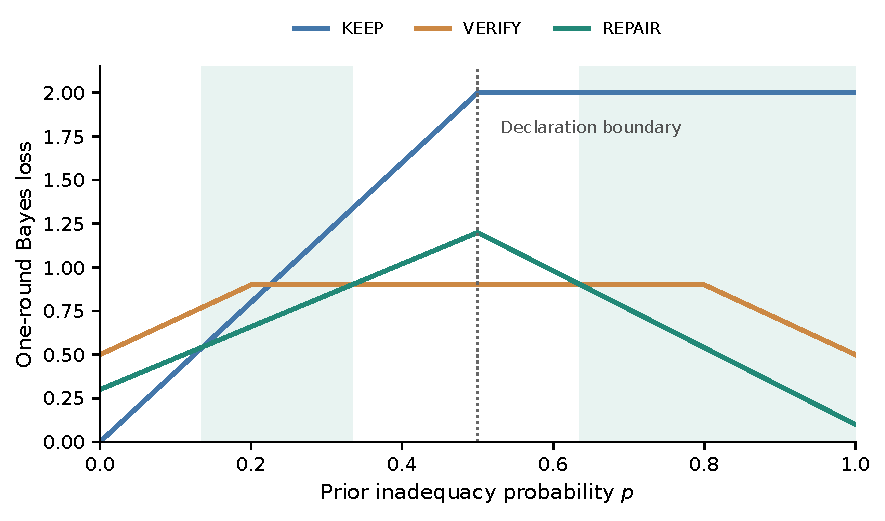
\includegraphics[width=.92\linewidth]{figures/disconnected_region.pdf}
\caption{Exact one-round action values. Shading marks the two repair intervals.
The dotted line is the declaration boundary, not an action constraint for the
joint controller. The lower repair interval lies entirely below that boundary.}
\label{fig:counter}
\end{figure}

\subsection{Robustness beyond one parameter point}
\begin{proposition}[Finite-horizon perturbation certificate]
\label{prop:robust}
Consider two models with the same finite environment, states, actions,
observation alphabet, and terminal decision sets. Suppose corresponding kernel
rows differ by at most $\epsilon_Q$ in total variation, stage costs differ by
at most $\epsilon_\ell$, and terminal costs differ by at most $\epsilon_L$.
Both stage and terminal costs are bounded by $L_{\max}$ and $L_B$, respectively.
For any fixed horizon-$h$ policy tree, and hence for an optimal value or a
root-action-constrained optimal value, the absolute value difference is at most
\begin{equation}
\mathcal E_h=
h\epsilon_\ell+\epsilon_L+
\epsilon_Q\left\{L_{\max}\frac{h(h+1)}2+hL_B\right\}.
\label{eq:robustbound}
\end{equation}
A unique action with gap $g>2\mathcal E_h$ remains uniquely optimal.
\end{proposition}
\begin{proof}
Condition on the same environment and couple corresponding observable events
maximally while histories agree. The probability that histories differ by the
end of round $t$ is at most $t\epsilon_Q$. The round-$t$ loss difference is
bounded by $\epsilon_\ell+tL_{\max}\epsilon_Q$ for $t=1,\ldots,h$; the terminal
difference is at most $\epsilon_L+hL_B\epsilon_Q$. Summation gives
\eqref{eq:robustbound}. The bound is uniform over policy trees. Taking minima
over the same feasible set preserves it, including when the first action is
fixed. Two action values can move toward one another by at most
$2\mathcal E_h$.
\end{proof}
At $p=1/4$, the strict repair margin is $3/20$. Continuity or the explicit bound
therefore gives a neighborhood of costs and full-support channel probabilities
where early repair remains uniquely optimal. The prior is also separated from
the declaration boundary. Thus the phenomenon holds on a nonempty open
parameter set, not only at a rational point. This perturbation statement keeps
physical action sets fixed; it does not assert continuity across arbitrary
changes in belief-dependent gates.

\section{What information can eliminate}
\label{sec:information}
\subsection{Blackwell improvement for a pure information action}
\begin{proposition}[Standard information monotonicity]
\label{prop:blackwell}
Replace a pure verification channel $P$ by $\widetilde P$ on the same hidden
environment, where $P=\widetilde P G$ for an environment-independent stochastic
garbling matrix $G$. Suppose verification has the same environment-wise cost
in both models, independent of its signal, and leaves the visible state unchanged
(or makes the same deterministic budget transition); all other primitives are
unchanged. Then the unrestricted optimal
Bayes loss cannot increase, at any finite horizon or initial belief.
\end{proposition}
\begin{proof}
After each fine-channel observation, a controller can sample the garbling and
run any coarse-channel policy on the resulting fictitious coarse history. Its
joint law of environments, coarse observations, actions, states, and losses
matches that in the coarse model. The fine model admits this randomized policy,
and a deterministic optimum is no worse. Taking the infimum over coarse policies
proves the result.
\end{proof}
This is the usual experiment-comparison argument \citep{blackwell1953}.
It compares total optimal value, not a static ranking of arbitrary interventions.
Changing the representation, state transition, or verification cost violates
the comparison's assumptions. Also, a gate based on the full posterior can
change which actions are permitted after refinement, so the same simulation
argument does not automatically prove monotonicity of the gated optimum.

\subsection{An informative gate need not have a linear cost}
Augment the binary family of Proposition~\ref{prop:noinfo} with a repeatable
verification action. Each verification consumes a round, leaves the old
representation in place, incurs its old task loss plus $c_v>0$, and yields an
independent observation from $P_i$ under environment $i$. Assume a finite
alphabet, distinct full-support $P_0,P_1$, deterministic repair, and no
post-repair information. There is no fallback or deferral. Keep and repair
retain their earlier meanings and costs, including the symmetric terminal cost.
All parameters are fixed as $T$ increases.

For $0<p<1$, define
\begin{equation}
\rho=\sum_y\sqrt{P_0(y)P_1(y)}<1,\qquad \beta=-\log\rho>0.
\end{equation}
Consider the following feasible gated policy: verify exactly $n\le T-1$ times,
estimate the environment by the posterior MAP rule, repair if it estimates
$I=1$, otherwise keep, and then execute tasks to the horizon. Report the
adequacy label implied by the inferred environment and the final representation.
On a posterior tie, choose $I=1$, which is gate-feasible.

\begin{theorem}[Finite bound and logarithmic gate-cost upper bound]
\label{thm:log}
The preceding policy satisfies
\begin{equation}
J_T(\pi_n)\le
n(pr+c_v)+c_r+
\bigl[(T-n)\max(r,s)+\lambda\bigr]\sqrt{p(1-p)}e^{-\beta n}.
\label{eq:testingbound}
\end{equation}
For all sufficiently large $T$, choose
$n_T=\lceil2\log T/\beta\rceil\le T-1$. Then
\begin{equation}
0\le V_T^G(p)-V_T(p)\le J_T(\pi_{n_T})=O(\log T).
\label{eq:logbound}
\end{equation}
Consequently, a lower bound $cT-C$ with fixed $c>0$ cannot hold for this
informative family for all sufficiently large horizons.
\end{theorem}
\begin{proof}
Let $z$ be the length-$n$ verification transcript. The Bayes MAP error is
\begin{align*}
\epsilon_n&=\sum_z\min\{(1-p)P_0^n(z),\,pP_1^n(z)\}\\
&\le \sqrt{p(1-p)}\sum_z\sqrt{P_0^n(z)P_1^n(z)}
=\sqrt{p(1-p)}\rho^n,
\end{align*}
using $\min(a,b)\le\sqrt{ab}$ and independence.
The verification phase has expected cost $n(pr+c_v)$. There is at most one
repair costing $c_r$. If the MAP decision is correct, the selected
representation has zero remaining task loss; if it is wrong, the loss per
remaining round is at most $\max(r,s)$. The terminal error probability is
$\epsilon_n$, because the chosen representation's label agrees with the
declaration exactly when the environment estimate is correct. This proves
\eqref{eq:testingbound}. A repair occurs only at a posterior at least $1/2$, so
the policy is gate-feasible. With $n_T$ the exponential term is at most $T^{-2}$,
and the first term grows at most logarithmically. Finally $V_T\ge0$ and
$V_T^G\le J_T(\pi_{n_T})$ give \eqref{eq:logbound}.
\end{proof}

The theorem is an upper bound, not a matching characterization of the gate gap.
The gap may be bounded or zero in other instances. The bound also does not
extend to a fixed verification budget, unidentifiable channels, costs growing
with $T$, or repairs with nonzero residual loss in their intended environments
without further analysis.

For numerical illustration, we evaluate fixed-prefix policies exactly using
binomial counts with $p=3/10$, $P_0(Y=1)=1/5$, $P_1(Y=1)=4/5$, $r=2$,
$s=1/2$, $c_r=1$, $c_v=1/4$, and $\lambda=1$. For each plotted horizon, we
minimize over $0\le n\le\min(100,T-1)$. This is the best \emph{tested prefix},
not the unrestricted gated optimum. The environment oracle has loss $pc_r=3/10$
for the reported horizons, and
$J_T(\pi_n)-3/10$ is a valid upper bound on the gate gap.

\begin{figure}[ht]
\centering
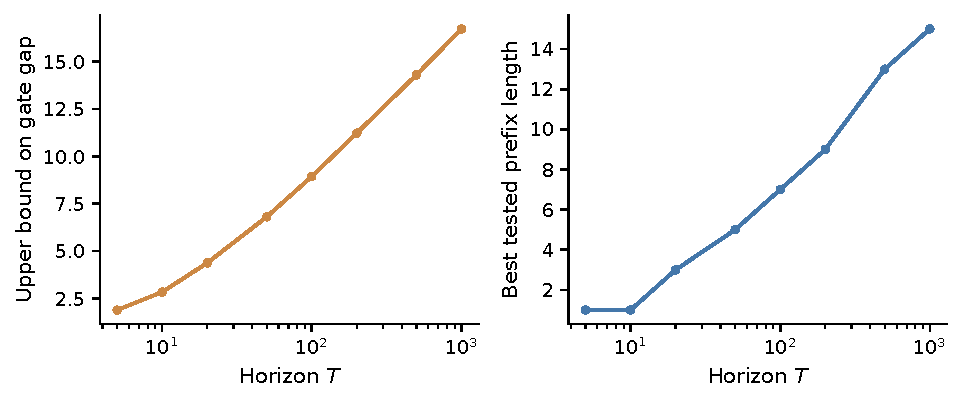
\includegraphics[width=.94\linewidth]{figures/informative_gate_bound.pdf}
\caption{A constructive upper bound when verification is repeatable and
identifiable. Left: tested fixed-prefix policy cost minus the oracle lower
bound. Right: its selected prefix length. These are not measurements of the
exact gated optimum at the large horizons.}
\label{fig:log}
\end{figure}

\subsection{Why the two boundaries coexist}
Equation~\eqref{eq:linear} concerns a controller that cannot acquire new
environment evidence. Equation~\eqref{eq:logbound} concerns one that can repeatedly
buy informative evidence. The former does not imply a universal linear
separation principle, and the latter does not remove the finite-horizon
counterexample of Theorem~\ref{thm:counter}. A short deadline, the task cost of
verification, and what repair makes observable can all influence the optimal
sequence. They must be compared under one explicit action and loss contract.

\section{Experiments and independent computation}
\label{sec:experiments}
All experiments are specified finite models. Bayes values and posterior updates
use Python rational arithmetic. Certification likelihood scores and count-lattice
probabilities use double precision with stable binomial tails. No Monte Carlo
experiment, participant study, or learned kernel is reported.

\subsection{Old-label certification and finite accounting}
The certification configuration uses \eqref{eq:example}, $q=0.8$,
$\kappa_i=0.3$, $\delta=0.05$, $H=2400$, $N=2000$, and $R=24$.
These finite budgets are explicit; they are not obtained by substituting
$\delta=0.05$ into the asymptotic sufficient schedule $H_\delta$.
Both policies use $\beta=\log480$. The joint race permits every decoder and
the separated race permits only constant ones. The factorized implementation
uses the same first-decoder tie rule as exhaustive search.

The evaluator propagates probability mass on Bernoulli count states $(n,u)$.
It checks eligibility also at $n=N$. An unresolved history incurs $g_iH$
and uses the pre-history maximum-likelihood old label. A stop at $n$ incurs
conditional expected cost
\[
g_i n+\kappa_i\frac{1-(1-q)^R}{q}
+(1-q)^R g_i(H-n-R).
\]
All-failed separated histories retain their committed answer. Joint histories
use a pre-history fallback. On each possible success time the remaining
post count is evaluated separately; replacing repair duration by its
expectation would not give the same terminal error.

\begin{table}[ht]
\centering\small\begin{tabular}{llrrrr}
\toprule
Policy & Env. & Cost & $\mathbb E N_P$ & Error & Timeout\\
\midrule
Joint & $E_1$ & 13.509374 & 13.134374 & 4.15e-18 & 8.71e-152\\
Joint & $E_2$ & 28.562326 & 28.187326 & 1.54e-03 & 2.45e-73\\
Joint & $E_3$ & 21.486990 & 21.111990 & 1.67e-03 & 1.82e-73\\
Certify first & $E_1$ & 306.420695 & 306.042190 & 1.91e-03 & 8.77e-06\\
Certify first & $E_2$ & 28.648038 & 28.273038 & 1.23e-05 & 3.44e-73\\
Certify first & $E_3$ & 309.903293 & 309.524760 & 3.57e-03 & 8.84e-06\\
\bottomrule
\end{tabular}

\caption{Finite count-lattice evaluation of old-label certification. Displayed
errors and timeout masses are floating-point values. Every total cost includes
failed attempts and unrepaired tails.}\label{tab:finite}
\end{table}
Every directly evaluated error is below $0.05$, and every conservative bound
from Section~\ref{sec:finite-deadline} with the nearest-mean error bound is
below $0.01251$. In $E_1$ the costs are $13.509374$ and $306.420695$, giving
a finite ratio $22.682079$ rather than the asymptotic ratio $25.026980$.
The improvement varies across environments. The $E_1$ joint unresolved
mass is approximately $8.71\times10^{-152}$. Numerical total-mass residuals
around $10^{-16}$ are reported separately and are not substituted for this
tail probability.

\begin{figure}[ht]
\centering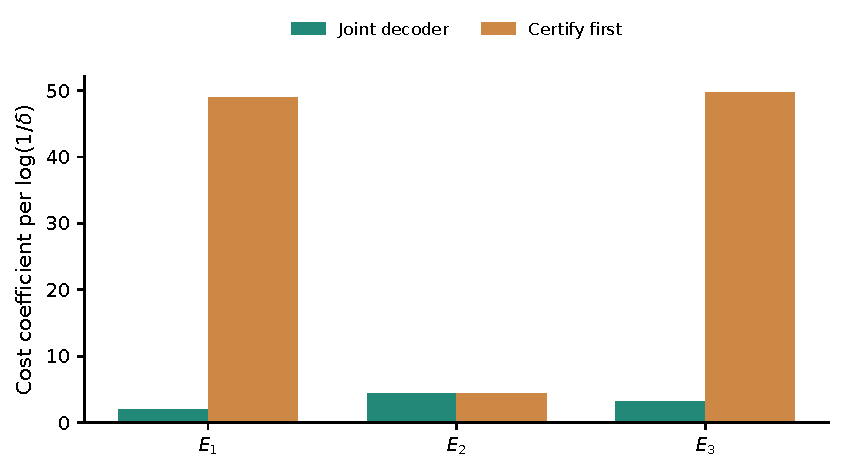
\includegraphics[width=.82\linewidth]{figures/certification_coefficients.pdf}
\caption{Fixed-instance asymptotic coefficients in the three-environment
example. Bars compare policy classes under the same old-label contract.}
\label{fig:coefficients}
\end{figure}

\subsection{A finite-deadline boundary of free post information}
For \eqref{eq:shrinking-example}, we evaluate the proved lower bound
\eqref{eq:deadline-cost-lower} at
$L_\delta=2,4,8,16,32,64,128,256$, using $H=L_\delta^2$.
These curves are analytic lower-bound evaluations; no purported exact
large-horizon certification optimizer is run. In $E_1$ the normalized bound
approaches the separated coefficient $48.9931965$, as proved by
Theorem~\ref{thm:collapse}. Every frozen post experiment has a universal
decoder, but the varying family has this positive leading coefficient.

\begin{figure}[ht]
\centering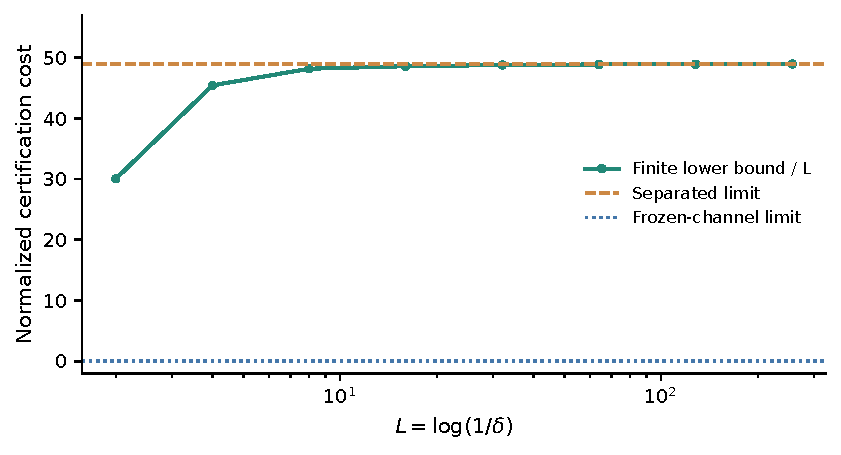
\includegraphics[width=.83\linewidth]{figures/shrinking_channel.pdf}
\caption{For $E_1$, finite information lower bound divided by $L_\delta$
along the shrinking-channel family, compared with its separated limit.
The zero line is the coefficient obtained when any one of the distinct post
experiments is frozen before sending the confidence level to zero.}
\label{fig:shrinking}
\end{figure}

\subsection{Current-label control in the original three-environment fixture}
This separate Bayes fixture has environments adequate, repairable, and
unrepairable, prior $(0.6,0.25,0.15)$, horizon $T=6$, and symmetric terminal
penalty $\lambda=0.5$. Old and new labels are $(1,0,0)$ and $(1,1,0)$;
their ordinary task costs are $(0,0.5,0.5)$ and $(0,0,0.5)$.
Every action takes one slot. In old mode, \KEEP{} has no information,
\VERIFY{} adds $0.08$ to the old task loss and yields Bernoulli means
$(0.2,0.8,0.8)$, and \REPAIR{} adds $0.2$ to old task loss and succeeds
with probability $0.8$ in every environment. Failure leaves the old mode
available for another attempt. The repair affects the \emph{next} task.
New-mode tasks yield Bernoulli means $(0.1,0.1,0.9)$.
Fallback costs $0.12$ per round, gives no information, and preserves whether
the installed representation is old or new. There are four visible modes.

The original gate restricts \REPAIR{} only, at posterior threshold $0.95$;
fallback remains available. This is neither the old-label commitment class
nor exactly the two-action gate definition used for the binary theorems.
Both its action set and its threshold are recorded in the model.
\begin{table}[ht]
\centering\small\begin{tabular}{lllrrr}
\toprule
Policy & Bayes cost & First action & $e_1$ & $e_2$ & $e_3$\\
\midrule
joint & 0.73146152 & repair & 0.036824 & 0.036824 & 0.017384\\
gate\_095 & 0.83414400 & verify & 0.232000 & 0.072000 & 0.072000\\
no\_repair & 0.83414400 & verify & 0.232000 & 0.072000 & 0.072000\\
\bottomrule
\end{tabular}

\caption{Exact current-label Bayes fixture, rounded for display.
The $e_i$ columns are conditional terminal errors under the same implemented
policy; no uniform $\delta$ constraint is imposed.}\label{tab:original-bayes}
\end{table}
The joint cost is exactly $9143269/12500000=0.73146152$; the two restricted
costs are $26067/31250=0.834144$. Initial actions are repair and verify,
respectively. Conditional errors agree with the independently reconstructed
original values.

A threshold sweep also yields $0.834144$ at threshold $0.5$ for this same
repair-only gate. Thus the default gap is not solely an artifact of imposing
$0.95$. The sweep evaluates explicit alternative restrictions and does not
turn a posterior gate into a frequentist confidence guarantee.

One-at-a-time sensitivity varies repair fee over $0,0.1,0.2,0.4,0.8$,
success probability over $0,0.2,0.5,0.8,1$, verification accuracy over
$0.5,0.65,0.8,0.95,1$, and horizon over $1,2,4,6,8$. All values and
first actions are in Appendix~\ref{app:original-sensitivity}.
The maximum difference from the supplied source archive's cost and error
columns is approximately $2.3\times10^{-13}$. Timeout residuals are treated
separately as described above.

\begin{figure}[ht]
\centering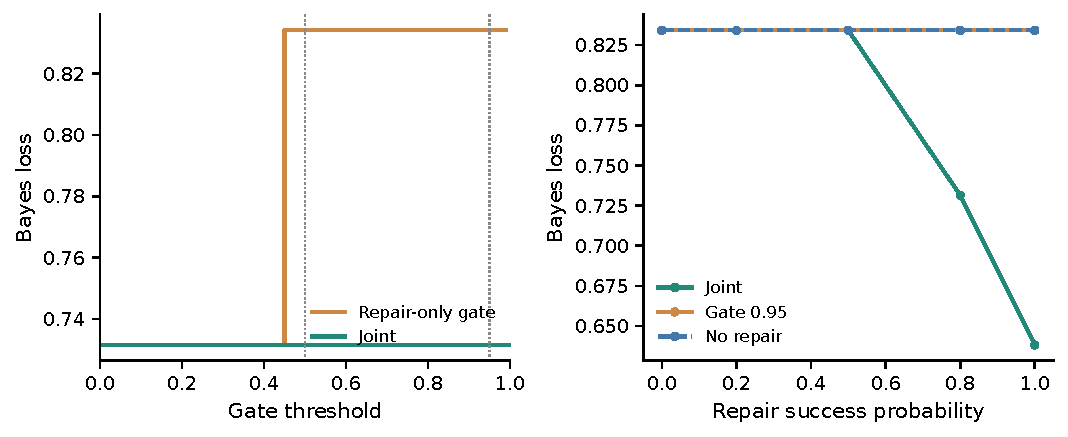
\includegraphics[width=.95\linewidth]{figures/original_sensitivity.pdf}
\caption{Current-label fixture. Left: repair-only gate as its threshold
varies, with unrestricted value as a reference. Right: values as repair success
varies at the original $0.95$ gate. Policies share all other primitives
within each comparison.}\label{fig:original-sensitivity}
\end{figure}

\subsection{Binary families and repair-region geometry}
Nine binary configurations retain the finite-horizon development:
F0 fixes the representation; F1 is the no-information benchmark;
F2 uses perfect verification; F3 uses full-support noisy verification;
F4 allows fallback and deferral; F5 has one repair attempt with success
probabilities $(3/4,1/2)$; F6 adds passive post information;
F7 is unidentifiable; and F8 is the exact one-round two-region example.
Complete rational parameters are stored in the configurations.
Unlike the three-environment fixture, these repairs affect the current task.
For F0--F7 verification retains old task loss in addition to its price.
For F8 and the repair-region sweep it replaces the round's ordinary task.
No comparison changes this convention between policies.

The joint and gate policies optimize their respective menus exactly.
Stage-myopic minimizes immediate cost; greedy-VOI minimizes immediate cost
plus the one-action terminal Bayes risk. Verify-then-act verifies once initially
and subsequently disables verification. Never-repair retains other actions;
always-repair forces the first repair and then optimizes. All use the same
optimal terminal declaration. The environment oracle knows the true index
only to provide a lower bound.
\begin{table}[ht]
\centering\small\begin{tabular}{lrrrrr}
\toprule
Instance & Oracle & Joint & Gate & Myopic & Gate gap\\
\midrule
F0 & 2.4000 & 3.0000 & 3.0000 & 3.0000 & 0.0000\\
F1 & 0.3000 & 4.8000 & 6.3000 & 6.3000 & 1.5000\\
F2 & 0.0300 & 1.1200 & 1.1300 & 1.1200 & 0.0100\\
F3 & 0.0300 & 1.4000 & 2.1300 & 1.4000 & 0.7300\\
F4 & 0.3000 & 2.6400 & 2.6400 & 3.6000 & 0.0000\\
F5 & 0.7200 & 2.3075 & 2.6520 & 2.3700 & 0.3445\\
F6 & 0.0300 & 0.9466 & 1.9290 & 0.9466 & 0.9825\\
F7 & 0.7800 & 1.9750 & 3.6000 & 1.9750 & 1.6250\\
F8 & 0.0250 & 0.7500 & 0.9000 & 0.7500 & 0.1500\\
\bottomrule
\end{tabular}

\caption{Binary Bayes benchmarks. Exact fractions and all seven policy
columns are provided in the CSV. A positive gate gap is not universal.}
\label{tab:benchmark}
\end{table}
F1 gives the exact gap $3/2$ and F8 the noisy gap $3/20$.
F4 has equal joint and gate values. Comparing F3 with F6, passive information
reduces joint loss from $1.4$ to $0.94656$ and gate loss from $2.13$ to
$1.92904$, while their gap increases. Better information therefore need not
reduce the difference between these two policy classes.

\begin{figure}[ht]
\centering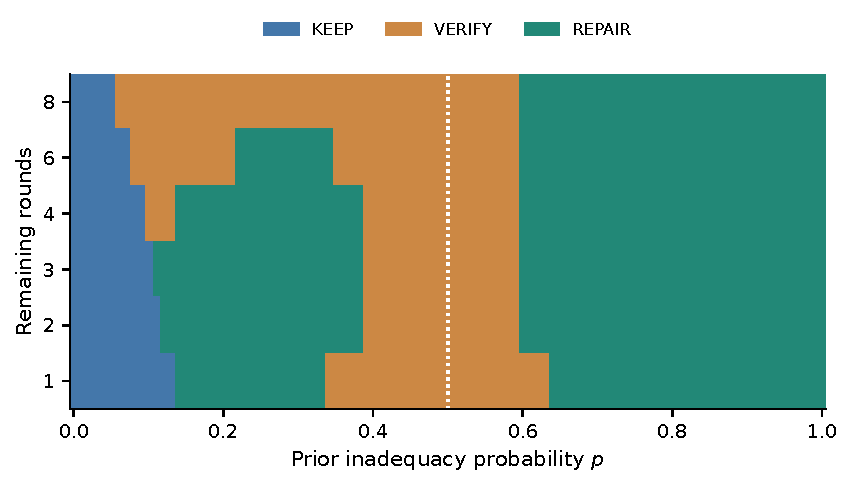
\includegraphics[width=.88\linewidth]{figures/horizon_regions.pdf}
\caption{Exact actions on 101 rational priors at six horizons.
Interpolation between sampled priors is illustrative; only the one-round
boundaries in Theorem~\ref{thm:counter} have the stated analytic endpoints.}
\label{fig:regions}
\end{figure}
\begin{figure}[ht]
\centering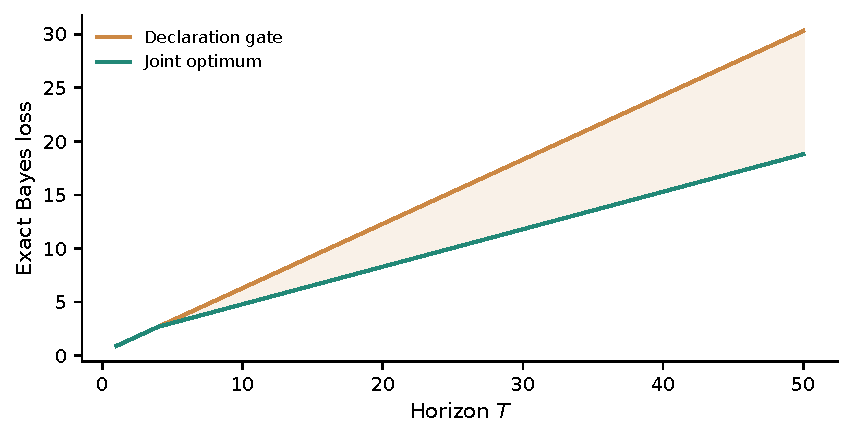
\includegraphics[width=.84\linewidth]{figures/no_information_gap.pdf}
\caption{The exact no-information gap is $\max(0,T/4-1)$ at the F1 parameters.
All displayed values agree with the rational solver.}\label{fig:noinfo}
\end{figure}
\begin{figure}[ht]
\centering
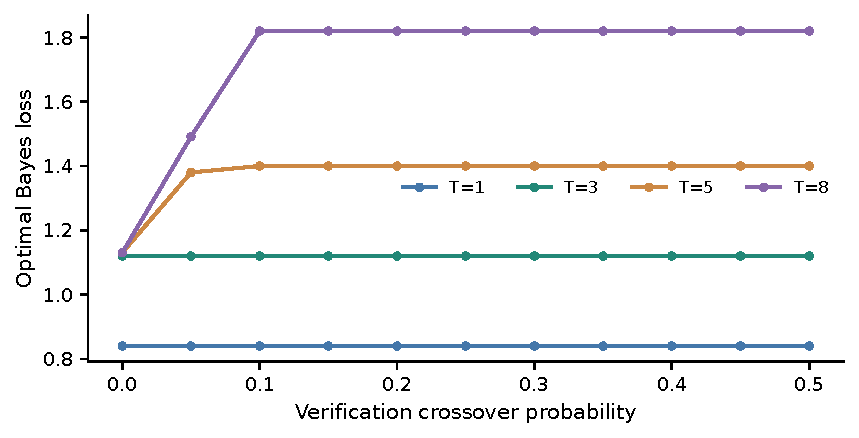
\includegraphics[width=.82\linewidth]{figures/blackwell.pdf}\\[5pt]
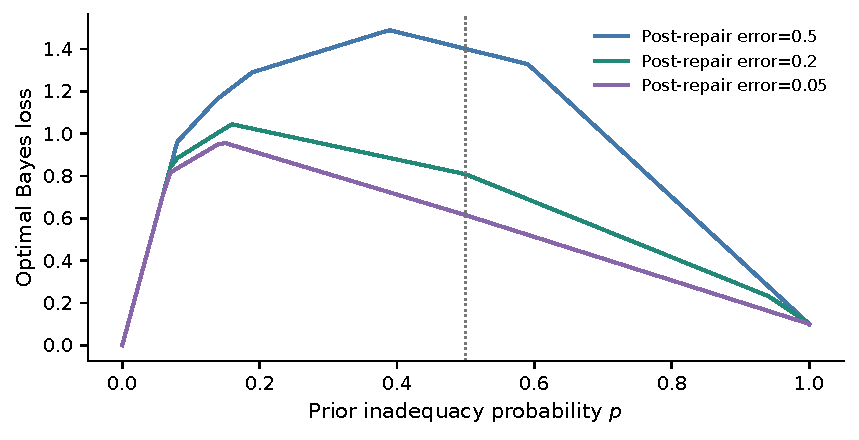
\includegraphics[width=.82\linewidth]{figures/post_information.pdf}
\caption{Top: unrestricted value under a pure verification channel comparison
at fixed costs. Bottom: values for three passive post-repair channels.
These are finite value calculations, not general monotonicity claims for
the gate gap.}\label{fig:information}
\end{figure}

The long-horizon fixed-prefix illustration in Figure~\ref{fig:log}
tests $0\le n\le\min(100,T-1)$. At $T=1000$ it selects $n=15$ and
has loss approximately $17.02328$. Subtracting the oracle $0.3$ gives
a valid gate-gap upper bound $16.72328$, not the optimal gated value.

\subsection{Independent checks and computational limits}
The policy-tree enumerator never updates a posterior or invokes the Bellman
solver. It enumerates environment-wise loss vectors for all deterministic
trees, retaining duplicates, and then minimizes their prior inner products.
All 20 binary prior--horizon comparisons and all 12 three-environment
comparisons have exactly zero rational difference. The largest enumerated
tree family has 61,872 policies.

The 32-test suite checks exact thresholds and endpoints, factorized versus
enumerated decoder coefficients and eligibility, equality-at-threshold ties,
global decoder tie breaking, the two finite protocol implementations,
visible success information, aggregation, multi-slot action completion,
fallback labels, asymmetric errors, abstention, serialization, gate menus,
and a $10^{-12}$-probability branch with $10^{12}$ loss. Tests of the new
structural formulas supplement their proofs; they do not establish
mathematical priority or formal verification.

For $N_b$ cached belief nodes, at most $A$ actions and $O$ joint observable
outcomes, Bellman computation uses $O(N_bAOK)$ rational operations, excluding
integer bit complexity. The number of nodes can grow exponentially in the
horizon. The supplied binary timing family grows from five cached nodes at
one round to 313 at twelve rounds; this is an instance-specific count.
An online factorized decoder check is polynomial in $K$, but a Bernoulli
count-lattice evaluator handles $O(N^2)$ histories, each with its own
eligibility and post-tail calculation. These are separate complexity claims.

\FloatBarrier
\section{Discussion and limitations}
\label{sec:discussion}
The old-label result makes repair useful as an information operation even
when the eventual answer remains about the obsolete representation. The useful
pre-repair answer is a decoder for the information available later. The
classwise bottleneck and surviving-set test make this answer structure
explicit and computationally manageable for a single online trajectory.

The fixed-instance coefficient depends on exact equality of post laws.
The finite-deadline bound supplies the missing quantitative qualification:
a nominally distinguishing channel may contribute too little information
within the available time. The shrinking-channel theorem demonstrates that
the leading advantage can disappear without any two post laws being exactly
equal at a finite confidence level. It also explains why finite experiments
should report actual post budgets rather than only the partition.

The current-label Bayes results answer a different operational question.
A declaration gate can forbid a uniquely optimal repair, and the cost of the
restriction depends on where the policy actually goes. A pairwise repair--keep
threshold need not remain a threshold when verification is available.
When repair has a fixed passive continuation, its terminal risk pieces bound
the number of disconnected regions regardless of the pre-repair policy's
complexity.

The following limits determine what can be inferred.
\begin{enumerate}
\item Models, costs, and candidate representations are known and finite.
The paper neither estimates unknown kernels nor learns a new representation
family. Exact risk-table realization alone imposes no additional control
structure.
\item The fixed-confidence coefficient assumes one pre channel, no return to
pre observations after entering repair, fixed environment-independent
success probability, and zero post cost. Positive post costs or multiple
controlled channels call for a new allocation analysis.
\item Environment-dependent success changes the information in repair outcomes,
so the random-decoder proof cannot be reused unchanged. For fixed
$q_i>0$, however, the expected attempts until success can still be bounded
by $1/q_i$. Informative outcomes alone do not prove that repair cost becomes
leading order.
\item The two-component Bayes repair bound requires a binary environment,
one specified deterministic irreversible repair, passive continuation, and
symmetric terminal error cost. The generic solver supports some cases,
such as stochastic repair, outside this theorem.
\item The $1/2$ declaration gate uses symmetric Bayes errors. An externally
imposed $0.95$ posterior gate is a different restriction. Neither is the
uniform fixed-confidence commitment requirement.
\item The logarithmic Bayes gate bound is an upper bound in a specified
zero-residual-loss family. No matching logarithmic lower bound or optimal
constant is asserted. The finite information lower bound is also not a
general solution of paid two-phase sensing.
\item Computational examples are small, synthetic, and deterministic.
Count-lattice certification sums use floating point, while the Bayes solver
uses exact rational values. Neither confirms a general theorem by experiment
nor establishes large-scale deployment performance.
\end{enumerate}

\paragraph{Further questions.}
A natural next theory problem charges observations on both sides of repair,
or chooses among several repairs with different post partitions and residual
task risks. Another imposes a meaningful constraint on representations,
such as a fixed feature or memory budget, and asks which additional control
structure follows. These questions are more specific than assuming that
representation change must create a fundamentally non-Markovian process.
A belief state remains sufficient for the finite known model considered here.

\section{Conclusion}
Repair can change which evidence must be collected before acting and how
later evidence is interpreted. In an ordered fixed-confidence experiment this
gives a decoder coefficient, a factorized computation, and a polynomial
likelihood-ratio policy. A finite-deadline lower bound identifies a regime in
which weakening post observations removes the coefficient advantage.
For current-label finite-horizon control, declaration gates have an exact
cost characterization, and a passive repair continuation bounds the topology
of repair regions. Explicit noisy examples and a reproducible implementation
make the distinction between certification and intervention checkable.

\paragraph{Reproducibility and computational assistance.}
The accompanying release contains the complete manuscript and proofs, LaTeX,
bibliography, exact Bayes solver, independent policy-tree enumerator, two
decoder implementations, frozen configurations, numerical outputs, and
figure-generation commands. The provided source archive for the earlier
manuscript contained LaTeX and generated outputs; its original Python
repository was not supplied. The integrated release uses the independently
reconstructed evaluators described here and does not represent the unavailable
repository as audited. Mathematical development, drafting, and programming
used AI assistance. This is a research draft, without a claim of formal proof
verification, peer-review acceptance, or confirmed priority over all related
literature. No participant data or private deployment logs are used.

\bibliographystyle{plainnat}
\bibliography{references}
\clearpage
\appendix
\section{Notation and theorem assumptions}
\begin{longtable}{p{.24\linewidth}p{.68\linewidth}}
\toprule
Symbol & Meaning\\
\midrule
$I,\cE,\mu$ & Fixed hidden environment, its finite set, and prior\\
$F_t,M_t,B_t$ & Representation, visible policy mode, and repair budget\\
$X_t,\cH_t$ & Visible control state and complete observable history\\
$\Theta_i(f),\Delta_i(f)$ & Reference-task adequacy and excess risk\\
$\mathsf K_i(y,x'\mid x,a)$ & Joint observation--successor kernel\\
$b_t,\Phi$ & Posterior on environments and its Bayes update\\
$T,h$ & Deployment horizon and remaining rounds\\
$V_h,\mathcal Q_h$ & Unrestricted optimal loss and action value\\
$G_h,V_h^G,W_h$ & Gate, gated loss, and their difference\\
$A_h$ & Joint-optimal Bellman loss advantage\\
$p_{\dec},p_{\inte}$ & Declaration and intervention boundaries when defined\\
$q_i(z),m_u$ & Passive post-repair transcript law and its distinct risk breakpoints\\
$\rho,\beta$ & Hellinger affinity and its negative logarithm for verification\\
\bottomrule
\end{longtable}

\begin{longtable}{p{.26\linewidth}p{.64\linewidth}}
\toprule
Result & Assumptions beyond the finite model\\
\midrule
Decoder coefficient & Assumption~\ref{ass:repair}; fixed instance and fully charged tails\\
Factorized race & Binary labels on a disjoint post-law partition\\
Shrinking-channel limit & Fixed pre laws and costs; $H_\delta\KL(Q_i^\delta\Vert Q_j^\delta)=o(L_\delta)$ for opposite labels\\
Gate-cost identity & Nonempty gate, identical terminal decisions and loss\\
No-information threshold & Binary labels reversed by deterministic repair;
no new information; symmetric terminal costs; only keep/repair\\
Repair-region bound & Binary environment; a fixed irreversible repair;
passive continuation; affine nonterminal cost; opposite repaired labels;
symmetric terminal costs\\
Two-region example & Explicit one-round parameters in Section~\ref{sec:counter}\\
Perturbation bound & Common finite spaces and physical action sets;
uniform kernel/cost perturbation bounds\\
Blackwell comparison & Pure information action, unchanged costs and state
transition, environment-independent garbling\\
Logarithmic gate bound & Repeatable independent full-support identifiable
verification; old-task cost during verification; deterministic repair;
zero task loss in the correctly selected mode; fixed parameters\\
\bottomrule
\end{longtable}
Each result has a proof in the main text. The tables specify their scope and
should not be read as extending one theorem to another experiment family.

\section{A complete noisy posterior calculation}
At the counterexample prior $p=1/4$, verification yields
\begin{align*}
\Pp(Y=1)&=\frac34\frac15+\frac14\frac45=\frac7{20},
&
\Pp(I=1\mid Y=1)&=\frac47,\\
\Pp(Y=0)&=\frac{13}{20},
&
\Pp(I=1\mid Y=0)&=\frac1{13}.
\end{align*}
The representation remains $f_0$, whose inadequate environment is $I=1$.
After $Y=1$, the optimal declaration is inadequate, with conditional loss
$2(3/7)=6/7$. After $Y=0$, it is adequate, with conditional loss $2/13$.
The expected terminal loss is
\[
\frac7{20}\frac67+\frac{13}{20}\frac2{13}=\frac25.
\]
Adding the verification cost $1/2$ gives $9/10$.
Repair costs $1/10$, changes the per-round expected task loss to
$(3/4)(1/5)=3/20$, and changes the label map. Its symmetric terminal risk is
still $2\min(1/4,3/4)=1/2$, so its total is $3/4$.
All task and terminal terms are accounted for.

\section{Asymmetric declarations and abstention}
For old labels $(1,0)$, define
\[
g_0(p)=\min\{\lambda_{\rm miss}p,\lambda_{\rm FA}(1-p)\}.
\]
After a label-reversing repair, the corresponding risk is
\[
g_1(p)=\min\{\lambda_{\rm miss}(1-p),\lambda_{\rm FA}p\}.
\]
With an abstention cost, include $\lambda_\bot$ as a third option in each
minimum. In the no-information family the two macro values are
$hpr+g_0(p)$ and $c_r+h(1-p)s+g_1(p)$.
They need not share a terminal term. Thus the symmetric closed-form threshold
cannot be carried over by merely substituting a new $p_{\dec}$.
One can instead partition $[0,1]$ at the breakpoints of $g_0,g_1$ and compare the
resulting affine expressions on each piece. The solver implements the full
terminal loss without this simplification.

\section{The scalar adequacy probability can lose necessary information}
Consider three environments, two representations, and one remaining round.
Old task losses are $(0,2,2)$; repaired task losses are $(1/5,0,3)$.
The labels are determined by whether these risks vanish. Repair costs $1/10$,
there are no observations, and both terminal error penalties equal $1/10$.
At beliefs $b=(1/2,1/2,0)$ and $b'=(1/2,0,1/2)$, the old inadequacy probability
is the same, namely $1/2$.

Under $b$, keep costs $1+1/20=21/20$ and repair costs
$1/10+1/10+1/20=1/4$. Under $b'$, keep still costs $21/20$, whereas
repair costs $1/10+1/10+3/2=17/10$; its current label is certainly inadequate,
so its terminal risk is zero. Thus the optimal action is repair at $b$ and keep
at $b'$. Proposition~\ref{prop:realize} realizes both loss tables by finite
representations with environment-independent visible outputs.
The scalar probability cannot be the general sufficient state.

\section{Independent policy-tree recurrence}
Let $\Gamma_0(x)=\{(L_i(x,d))_{i=1}^K:d\in\mathcal D(x)\}$, retaining
distinct policy labels even when their vectors coincide.
For an action $a$ and one selected continuation vector
$\alpha^{y,x'}\in\Gamma_{h-1}(x')$ at each observable event, define
\[
\alpha_i=\sum_{y,x'}\mathsf K_i(y,x'\mid x,a)
\left[\ell_i(x,a,y,x')+\alpha_i^{y,x'}\right].
\]
Enumerating every action and every such selection forms $\Gamma_h(x)$.
By conditioning on the first event, this lists all deterministic policy-tree
loss vectors. Therefore
\[
V_h(b,x)=\min_{\alpha\in\Gamma_h(x)}b^\top\alpha.
\]
This recurrence provides both the standard geometry argument and an independent
finite implementation that never computes a posterior. It is used only for the
unrestricted model; a belief-dependent gate would require checking tree
feasibility at each reached posterior.

\section{Exact prefix-policy calculation}
For a BSC with crossover $e$, write
\[
q_0(k)=\binom nk e^k(1-e)^{n-k},\qquad
q_1(k)=\binom nk (1-e)^k e^{n-k}.
\]
Let $\mathcal K_n=\{k:pq_1(k)\ge(1-p)q_0(k)\}$,
$e_0=\sum_{k\in\mathcal K_n}q_0(k)$, and
$e_1=\sum_{k\notin\mathcal K_n}q_1(k)$.
For $n\le T-1$, the fixed-prefix policy used in
Figure~\ref{fig:log} has exact cost
\begin{align*}
J_T(\pi_n)={}&n(pr+c_v)
 +(1-p)e_0[c_r+(T-n)s]\\
 &+p(1-e_1)c_r+pe_1(T-n)r
 +\lambda[(1-p)e_0+pe_1].
\end{align*}
Every term is evaluated with rational arithmetic before decimal export.
This is a direct evaluation of a feasible policy; the large-horizon experiment
does not run a purported exact POMDP solver at $T=1000$.

\section{Reproduction protocol and artifact map}
From the project root, \texttt{python3 scripts/reproduce.py} runs the test suite,
regenerates frozen computations, creates vector figures, and compiles the
manuscript using \texttt{latexmk}. Without a TeX installation, use the explicit
\texttt{--skip-pdf} option. The exact solver itself needs only
Python's standard library. Figure generation requires NumPy and Matplotlib.
The manuscript uses ordinary LaTeX packages and BibTeX.

The source is organized into model validation, belief updates, exact Bellman
control, exhaustive enumeration, baseline evaluation, analytic formulas, and a
command-line interface. Configuration files specify rational parameters.
Result files include every table column, exact fractions, diagnostics, source
and model hashes, finite enumeration checks, timing measurements, and a complete
optimal policy DAG for the failed-repair instance. The generic model JSON stores
full joint kernels and terminal costs.

The tests verify implementation properties independently where possible.
Numerical sweeps verify finite instances, not general claims. The package does
not contain a proof-assistant formalization. General multiple-repair topology,
a tight noisy gate-gap asymptotic constant, and open-world representation
discovery remain outside the proved scope.

\section{Additional code validation for the three-environment example}
The test suite constructs the full explicit kernel for the preceding
three-environment example and checks both optimal actions without compressing
the belief to a scalar. It also checks that the model serialization preserves
exact probabilities and that an observed repair-success event changes the
posterior when success probabilities differ by environment. These tests guard
against two implementation shortcuts that would invalidate the stated model:
conditioning only on an observation token while ignoring the visible successor,
and replacing the environment belief by a single adequacy probability.

\section{Checked aggregation and multi-slot actions}
\label{app:adapters}
\begin{proposition}[A sufficient environment partition]
Suppose environments in each block have identical current labels, terminal
costs for every declaration, joint event probabilities, and task/direct
costs on every state--action--event triple. Then block posterior masses,
the visible state, and remaining horizon suffice for optimal Bayes control.
\end{proposition}
\begin{proof}
Within a block every likelihood and loss vector coordinate is identical.
Predictive event probabilities and expected costs therefore depend only on
block masses. Summing the individual Bayes update gives Bayes' rule on these
masses. The terminal minimum also depends only on them. Backward induction
proves value preservation. This is sufficient and makes no minimality claim.
\end{proof}
The implementation checks these equalities before constructing the quotient;
it rejects an invalid proposed merge.

Positive integer macro durations can be expressed without zero-time cycles.
Assume an action of duration $d(x,a)$ reveals its joint event at completion,
with a specified full-action cost, and cannot be interrupted.
\begin{proposition}[Duration expansion]
If an action is available only when $d(x,a)\le h$, its macro decision problem
is equivalent to a finite unit-slot problem with visible countdown states.
\end{proposition}
\begin{proof}
Augment each decision state with its remaining horizon. A duration-one action
uses the original completion kernel. A longer action first enters a countdown
state; intermediate transitions reveal only deterministic time advancement,
cost zero, and permit only continuation. Its last transition uses the original
joint event and charges its full cost exactly once. Filter actions that cannot
finish before the deadline. Every macro policy gives a unit policy by inserting
forced continuations, and every unit policy induces the corresponding macro
choices. The joint law at decision times, total costs, and terminal declaration
law coincide. Therefore their optimal values coincide.
\end{proof}
The adapter uses this completion convention explicitly. It does not assert
equivalence when observations arrive during the action or interruption is allowed.

\section{Finite count-lattice recurrence}
For a Bernoulli pre mean $p_i$, let $w_i(n,u)$ be active mass at count $(n,u)$
before the eligibility check. Initialize $w_i(0,0)=1$. Remove selected mass,
then propagate each unresolved cell by
\[
w_i(n+1,u)\mathrel{+}=(1-p_i)w_i(n,u),\qquad
w_i(n+1,u+1)\mathrel{+}=p_iw_i(n,u).
\]
At $n=N$ check eligibility first and charge every remaining unresolved cell.
The policy selects a decoder using all candidate likelihoods; the index $i$
in this recurrence is used only by the evaluator to compute that common
policy's performance.

After selection at $n$, success on attempt $r\le R$ has probability
$q(1-q)^{r-1}$ and leaves $H-n-r$ post observations. For a post mean $v_i$,
sum the binomial probabilities whose nearest class mean maps to the wrong
old label under the selected decoder. Midpoint ties use the lowest original
class index. The implementation accumulates small tails directly from a
large term using a probability-mass recurrence; subtraction from one is avoided
where it would erase a small tail. These are finite floating-point sums,
not certified interval bounds. Their normalization residual is stored separately.

\section{Original-fixture sensitivity table}
\label{app:original-sensitivity}
Every row changes only its named parameter from the three-environment
current-label fixture. The fixed-confidence theorem is not applied to
the rows with repair success zero.
\begin{center}\small\begin{tabular}{lrrrrl}
\toprule
Parameter & Setting & Joint & Gate & No repair & Action\\
\midrule
repair\_cost & 0 & 0.482416 & 0.834144 & 0.834144 & repair\\
repair\_cost & 0.1 & 0.607344 & 0.834144 & 0.834144 & repair\\
repair\_cost & 0.2 & 0.731462 & 0.834144 & 0.834144 & repair\\
repair\_cost & 0.4 & 0.834144 & 0.834144 & 0.834144 & verify\\
repair\_cost & 0.8 & 0.834144 & 0.834144 & 0.834144 & verify\\
repair\_success & 0 & 0.834144 & 0.834144 & 0.834144 & verify\\
repair\_success & 0.2 & 0.834144 & 0.834144 & 0.834144 & verify\\
repair\_success & 0.5 & 0.834144 & 0.834144 & 0.834144 & verify\\
repair\_success & 0.8 & 0.731462 & 0.834144 & 0.834144 & repair\\
repair\_success & 1 & 0.638146 & 0.834144 & 0.834144 & repair\\
verify\_accuracy & 0.5 & 0.731703 & 0.920000 & 0.920000 & repair\\
verify\_accuracy & 0.65 & 0.731703 & 0.920000 & 0.920000 & repair\\
verify\_accuracy & 0.8 & 0.731462 & 0.834144 & 0.834144 & repair\\
verify\_accuracy & 0.95 & 0.601000 & 0.601000 & 0.601000 & verify\\
verify\_accuracy & 1 & 0.520000 & 0.520000 & 0.520000 & verify\\
horizon & 1 & 0.320000 & 0.320000 & 0.320000 & fallback\\
horizon & 2 & 0.440000 & 0.440000 & 0.440000 & fallback\\
horizon & 4 & 0.658400 & 0.658400 & 0.658400 & verify\\
horizon & 6 & 0.731462 & 0.834144 & 0.834144 & repair\\
horizon & 8 & 0.773621 & 0.983863 & 0.983863 & repair\\
\bottomrule
\end{tabular}
\end{center}

\section{Code map and reproduction}
\label{app:code-map}
The project is self-contained. The complete release includes runnable code
and results; the separate arXiv source archive contains the LaTeX, bibliography,
and generated figures/tables required to compile this document.
{\small
\begin{longtable}{p{.44\linewidth}p{.48\linewidth}}
\toprule
File within \texttt{src/m2fh/} & Purpose\\\midrule
\texttt{model.py}, \texttt{belief.py} & Exact finite model and joint-event Bayes update\\
\texttt{solver.py}, \texttt{policies.py} & Control, policy restrictions, diagnostics and oracle\\
\texttt{enumerator.py} & Independent deterministic policy trees\\
\texttt{certification.py} & Bernoulli fixed-confidence finite protocol\\
\texttt{decoder\_structure.py} & Factorized coefficients and polynomial race\\
\texttt{deadline.py} & Finite information lower bound and shrinking family\\
\texttt{pdf\_fixture.py}, \texttt{families.py} & Explicit original and binary models\\
\texttt{aggregation.py}, \texttt{durations.py} & Checked quotient and macro-action expansion\\
\texttt{replay.py}, \texttt{cli.py} & Synthetic visible-event interface and command line\\
\bottomrule
\end{longtable}}
Run \texttt{python3 scripts/reproduce.py} from the project root after installing
the declared Python and TeX dependencies. Use \texttt{--skip-pdf} explicitly
when only computations are wanted. The script writes stage logs, a validation
report, source hashes, numerical tables, figures, and the final PDF.
\texttt{python3 scripts/package\_release.py} builds both release archives and
a SHA-256 file inventory. The generated tables in the arXiv archive permit
compilation without running Python.

The original supplied archive's output CSVs are preserved as reference data
in the provenance directory. They are not
presented as independently inspected original Python code. All results in
the integrated manuscript are regenerated by the included implementation.

\end{document}
